%%%%%%%%%%%%%%%%%%%%%%%%%%%%%%%%%%%%%%%%%%%%%%%%%%%%%%%%%%%%%%%%%
% Dissertacao de Mestrado / Dept Fisica, CFM, UFSC              %
% Lacerda@UFSC - 2013                                           %
%%%%%%%%%%%%%%%%%%%%%%%%%%%%%%%%%%%%%%%%%%%%%%%%%%%%%%%%%%%%%%%%%


%:::::::::::::::::::::::::::::::::::::::::::::::::::::::::::::::%
%                                                               %
%                          Capítulo 4                           %
%                                                               %
%:::::::::::::::::::::::::::::::::::::::::::::::::::::::::::::::%

%***************************************************************%
%                                                               %
%                       Testes com PCA                          %
%                                                               %
%***************************************************************%

\chapter{Aplicação a cubos de dados do CALIFA}
\label{sec:PCAaplic}

Com os dados e ferramentas apresentados nos capítulos anteriores estamos prontos para aplicar a Tomografia PCA a
galáxias do CALIFA. Como a PCA é uma técnica que calcula os eixos que, através da variância, melhor expandem a base de
dados, é natural que qualquer pré-processamento que modifique os espectros de entrada acarrete mudancas na variância
entre eles e portanto resulte num conjunto diferente de PCs. 

Durante nossas investigações fizemos uma série de testes com pré-processamentos e manipulações nos espectros
(normalização, remoção de cinemática, janelas diferentes em comprimento de onda, PCA das linhas de emissão, logarítmo do
fluxo, entre outros), verificando suas implicações no resultado. Neste capítulo comentaremos alguns {\em insights} que
tivemos nesse processo, e definiremos operações que julgamos adequadas a análise PCA de galáxias inteiras. Por fim
faremos uma espécie de engenharia reversa, estudando correlações entra PCs e propriedades derivadas da síntese de
populações estelares, o que nos auxilia na busca do sentido físico das PCs resultantes.

Todas as análises neste capítulo serão feitas usando a galáxia NGC 2916 (CALIFA 277), uma espiral de tipo Sbc (Figura
\ref{fig:K0277apresent}). A discussão detalhada desse caso particular serve de guia para os resultados para outras
galáxias de nossa amostra, apresentados no Capítulo \ref{sec:result}.

\section{PCA dos espectros observados: Efeitos de amplitude}
\label{sec:PCAaplic:norm}

Como exemplo inicial apresentamos as cinco primeiras PCs e seus respectivos tomogramas do cubo de espectros observados
da galáxia NGC 2916. Imagens SDSS e CALIFA dessa galáxia espiral podem ser vistas na Figura \ref{fig:K0277apresent},
enquanto a Figura \ref{fig:K0277ExampleSpectraFill} mostra o fluxo mínimo e máximo por comprimento de onda, dos
espectros observados desse objeto. No painel direito vemos o mesmo mas para os espectros observados normalizados.

\begin{figure}
    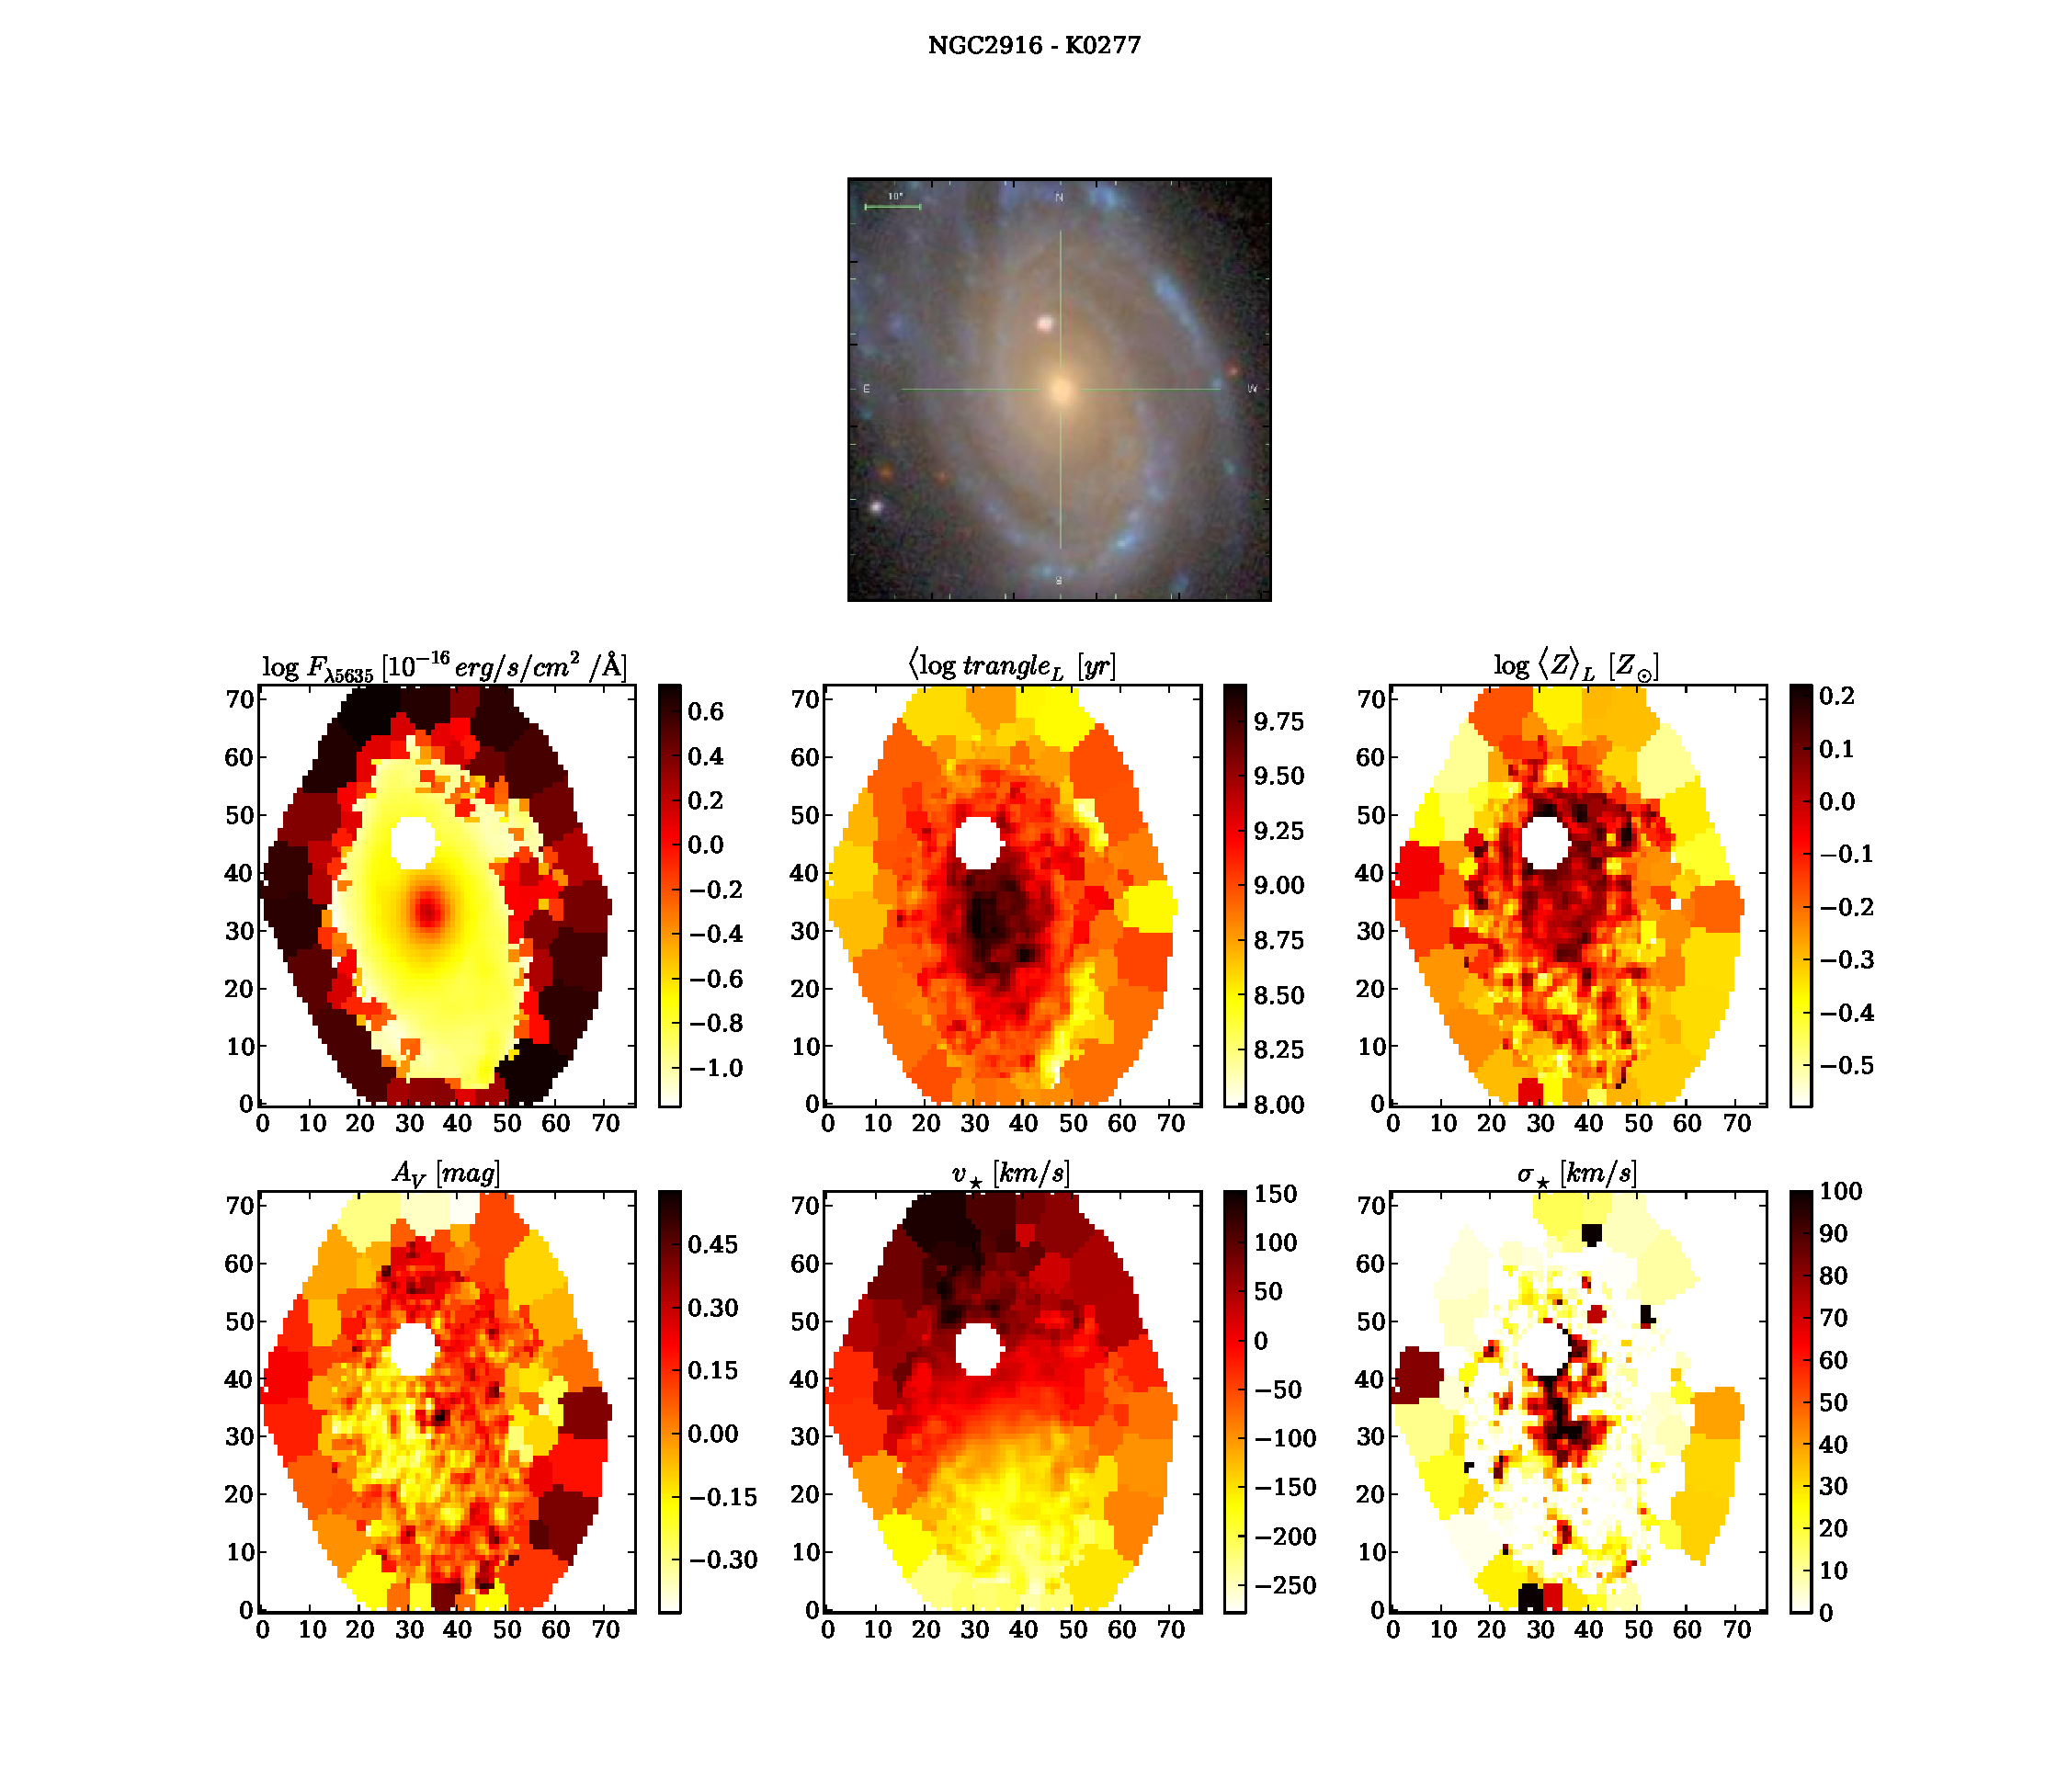
\includegraphics[width=1.\textwidth]{figuras/K0277-apresent.pdf}
    \caption[Propriedades f\'isicas da gal\'axia NGC 2916 (CALIFA 277).]
    {Propriedades físicas da galáxia NGC 2916 (CALIFA 277). Na primeira linha a imagem do SDSS da galáxia. Na primeira
    imagem da segunda linha temos o valor do fluxo observado em 5635 \AA, usado para a normalização dos espectros de
    cada zona. Da segunda imagem da segunda linha em diante temos as propriedades físicas que serão correlacionadas com
    as PCs. São elas: \meanL{\log\ t}, $\log\ \meanL{Z}$, $A_V$, $v_{\star}$, $\sigma_{\star}$.}
    \label{fig:K0277apresent}
\end{figure}

\begin{figure}
	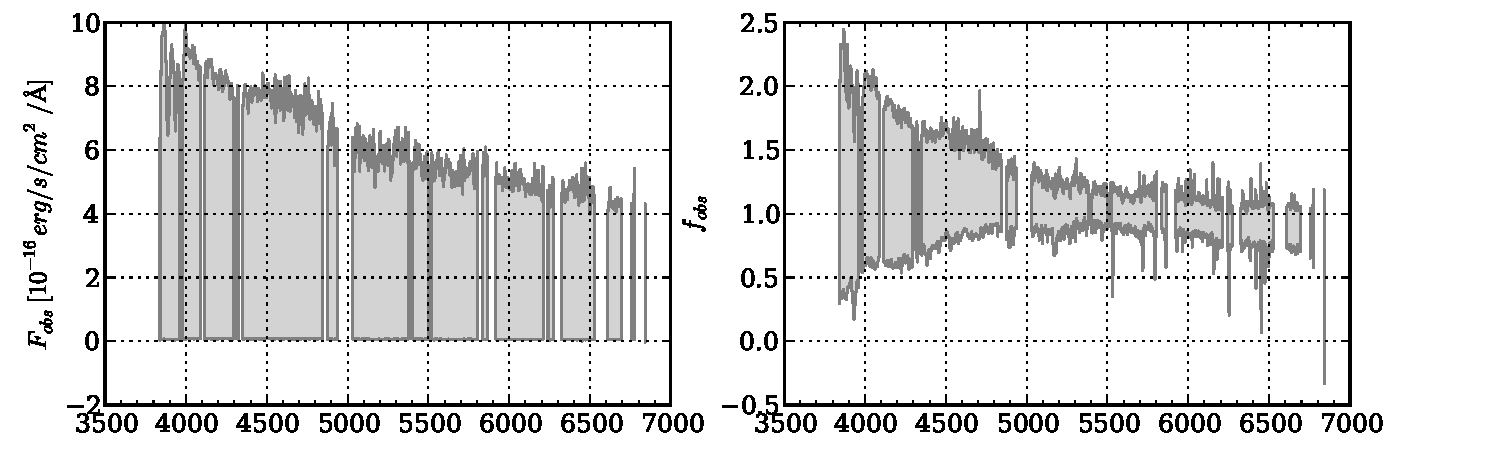
\includegraphics[width=1.\textwidth]{figuras/K0277-exampleSpectraFill.pdf}
    \caption[Máximo e mínimo de fluxo dos espectros da gal\'axia NGC 2916 (CALIFA 277).] 
    {Fluxo máximo e mínimo por comprimento de onda para o cubo de espectros da galáxia NGC 2916 (CALIFA 277). O painel à
    esquerda é para os espectros observados ($F_{obs}$) e o a direita para os espectros observados e normalizados pelo
    fluxo mediano na janela de $5635 \pm 45$ \AA ($f_{obs}$). Em destaque o 95\textsuperscript{\underline{o}} percentil.
    Todos os espectros do cubo já estão mascarados da mesma forma que o terceiro painel da Figura \ref{fig:checkmask}}
    \label{fig:K0277ExampleSpectraFill}
\end{figure}

A Figura \ref{fig:K0277tomofobs} apresenta os resultados da tomografia PCA para esse cubo de dados. O tomograma é
formado pelo ``peso'' da PC em cada zona (ver Equação \ref{eq:TomoPCA:tomogram2D}). O primeiro autoespectro lembra o
espectro médio (linha em cinza claro nos painéis à direita), embora muito mais azul. O segundo autoespectro se assemelha
com um espectro de população muito jovem. Com o auxilio de seu tomograma vemos que para as zonas mais internas da
galáxia (onde as populações são mais velhas, como vimos nas Figuras \ref{fig:mapaIdade} e \ref{fig:K0277apresent}) o seu
peso é negativo. De forma contrária, em regiões mais afastadas do núcleo, onde, para essa galáxia, parecem existir
algumas regiões H{\sc ii}, vemos que seu peso é positivo. A terceira componente parece mostrar um padrão de rotação, ao
mesmo tempo misturada com um fator de escala. Para que esse padrão de rotação ficasse visível tivemos que fazer um certo
tratamento no tomograma, mas falaremos mais sobre isso no final dessa seção. Da quarta componente em diante fica mais
complicado dizer o que cada uma representa. No final desse capítulo falaremos mais sobre como melhor interpretar as PCs
fisicamente.

Da mesma forma, fazemos a PCA para o mesmo cubo, mas com os espectros normalizados, i.e., reescalonando cada espectro de
modo que o fluxo médio na janela de $5590-5680$ \AA\ seja igual a 1. Daqui para frente vamos nos referir aos espectros
normalizados utilizando a letra $f$:
\begin{equation}
f_{obs} = \dfrac{F_{obs}}{F_{\lambda5635}}
\end{equation} 
\noindent A tomografia PCA desse cubo normalizado é mostrada na Figura \ref{fig:K0277tomofobsnorm}. À primeira vista os
resultados podem ser parecidos com o anterior deslocando uma componente acima, ou seja, a mesma PCA mas sem a primeira
PC. Mas essa é só uma primeira impressão. As propriedades físicas de uma galáxia geralmente possuem simetria radial ou
axial, sendo assim extremamente correlacionadas no espaço. Matematicamente, a maior fonte de variância nos espectros é
sua amplitude, aparecendo na forma de componente principal como visto na análise feita sem normalização. Essa componente
de escala, quando não suprimida, correlaciona-se com as propriedades físicas da galáxia, portanto, deixa sua assinatura
através de todas as PCs. Essa amplitude, que gera a primeira PC no caso sem normalização não adiciona nenhuma informação
qualitativa à análise das populações estelares, funcionando apenas como um fator de escala, afetando as componentes
seguintes. Esses vestígios de amplitude aparecem de forma mais evidente quando comparamos a PC3 no caso sem normalização
com a PC2 no caso com normalização. Podemos ver um claro padrão de rotação na PC2 da Figura \ref{fig:K0277tomofobsnorm}.
Com uma saturação na escala de cores no tomograma da PC3 da Figura \ref{fig:K0277tomofobs} diminuímos o efeito do fator
de escala ainda presente nessa componente, de modo que ficasse mais evidente o padrão de rotação. O espectro médio já é
a informação necessária que precisaríamos para entender esse fator de escala nas amplitudes dos espectros, portanto a
primeira componente para o caso sem normalização não trás informação adicional. Veremos a seguir que seu tomograma
também não trás maiores informações.

Imagine uma galáxia composta inteiramente pela mesma população estelar, em repouso, distribuídas da mesma maneira no
espaço. Ou seja, em qualquer ponto da galáxia o espectro é o mesmo. Uma PCA nessa galáxia hipotética não identificaria
nenhuma fonte de variancia, pois todos espectros são iguais ao espectro médio. Adicione então a essa galáxia uma função
de densidade de massa estelar em função do raio (ou, equivalentemente, um perfil de brilho superficial), permitindo que
de uma posição para outra a quantidade dessa determinada população se altera (mudando a intensidade da região). Uma
componente nova irá surgir na sua PCA, mostrando que existe uma variância agora numa componente de escala (amplitude)
nos espectros. Mas o que essa componente de escala nos diz sobre as propriedades da população estelar existente? Nada!
Essa componente seria um desperdício de variância para uma análise de populações estelares de uma galáxia.

No caso do CALIFA, com um campo abrangendo praticamente toda a galáxia, esse efeito de amplitude se acentua muito devido
ao brilho superficial mais intenso nas zonas centrais da galáxia em comparação com as mais afastadas, assim adicionando
uma grande variância descartável entres as zonas. Descartável pois não trazem informação nova para a nossa análise.
Essas diferenças em amplitude não nos dizem nada sobre as populações estelares. Comparemos agora a primeira PC do caso
sem normalização (Figuras \ref{fig:K0277tomofobs}) e a imagem mais à esquerda na Figura \ref{fig:K0277fobsnorm} formada
pelos fluxo para normalização por zona. Podemos notar que o primeiro autoespectro (e seu respectivo tomograma) no caso
sem normalização mostra exatamente esse fator de escala. Seu tomograma mostra que ela é claramente um fator de escala
(que pode ser considerado um fator de brilho, ou de amplitude, nos espectros).

Em suma, concluímos que é bem mais útil analisar espectros normalizados. Os trabalhos do grupo de J. Steiner não
utilizaram esse esquema de normalização, mas isso é muito provavelmente devido ao pequeno campo coberto por seus dados.
Nesse caso, as variações em amplitude são pequenas e não participam com um papel importante na analise. No caso do
CALIFA, contudo, os efeitos de amplitude são muito maiores, e complicam a interpretação dos resultados da PCA. Por esse
motivo, em nossas análises daqui para frente usaremos o cubo com os espectros normalizados.

\begin{figure}
    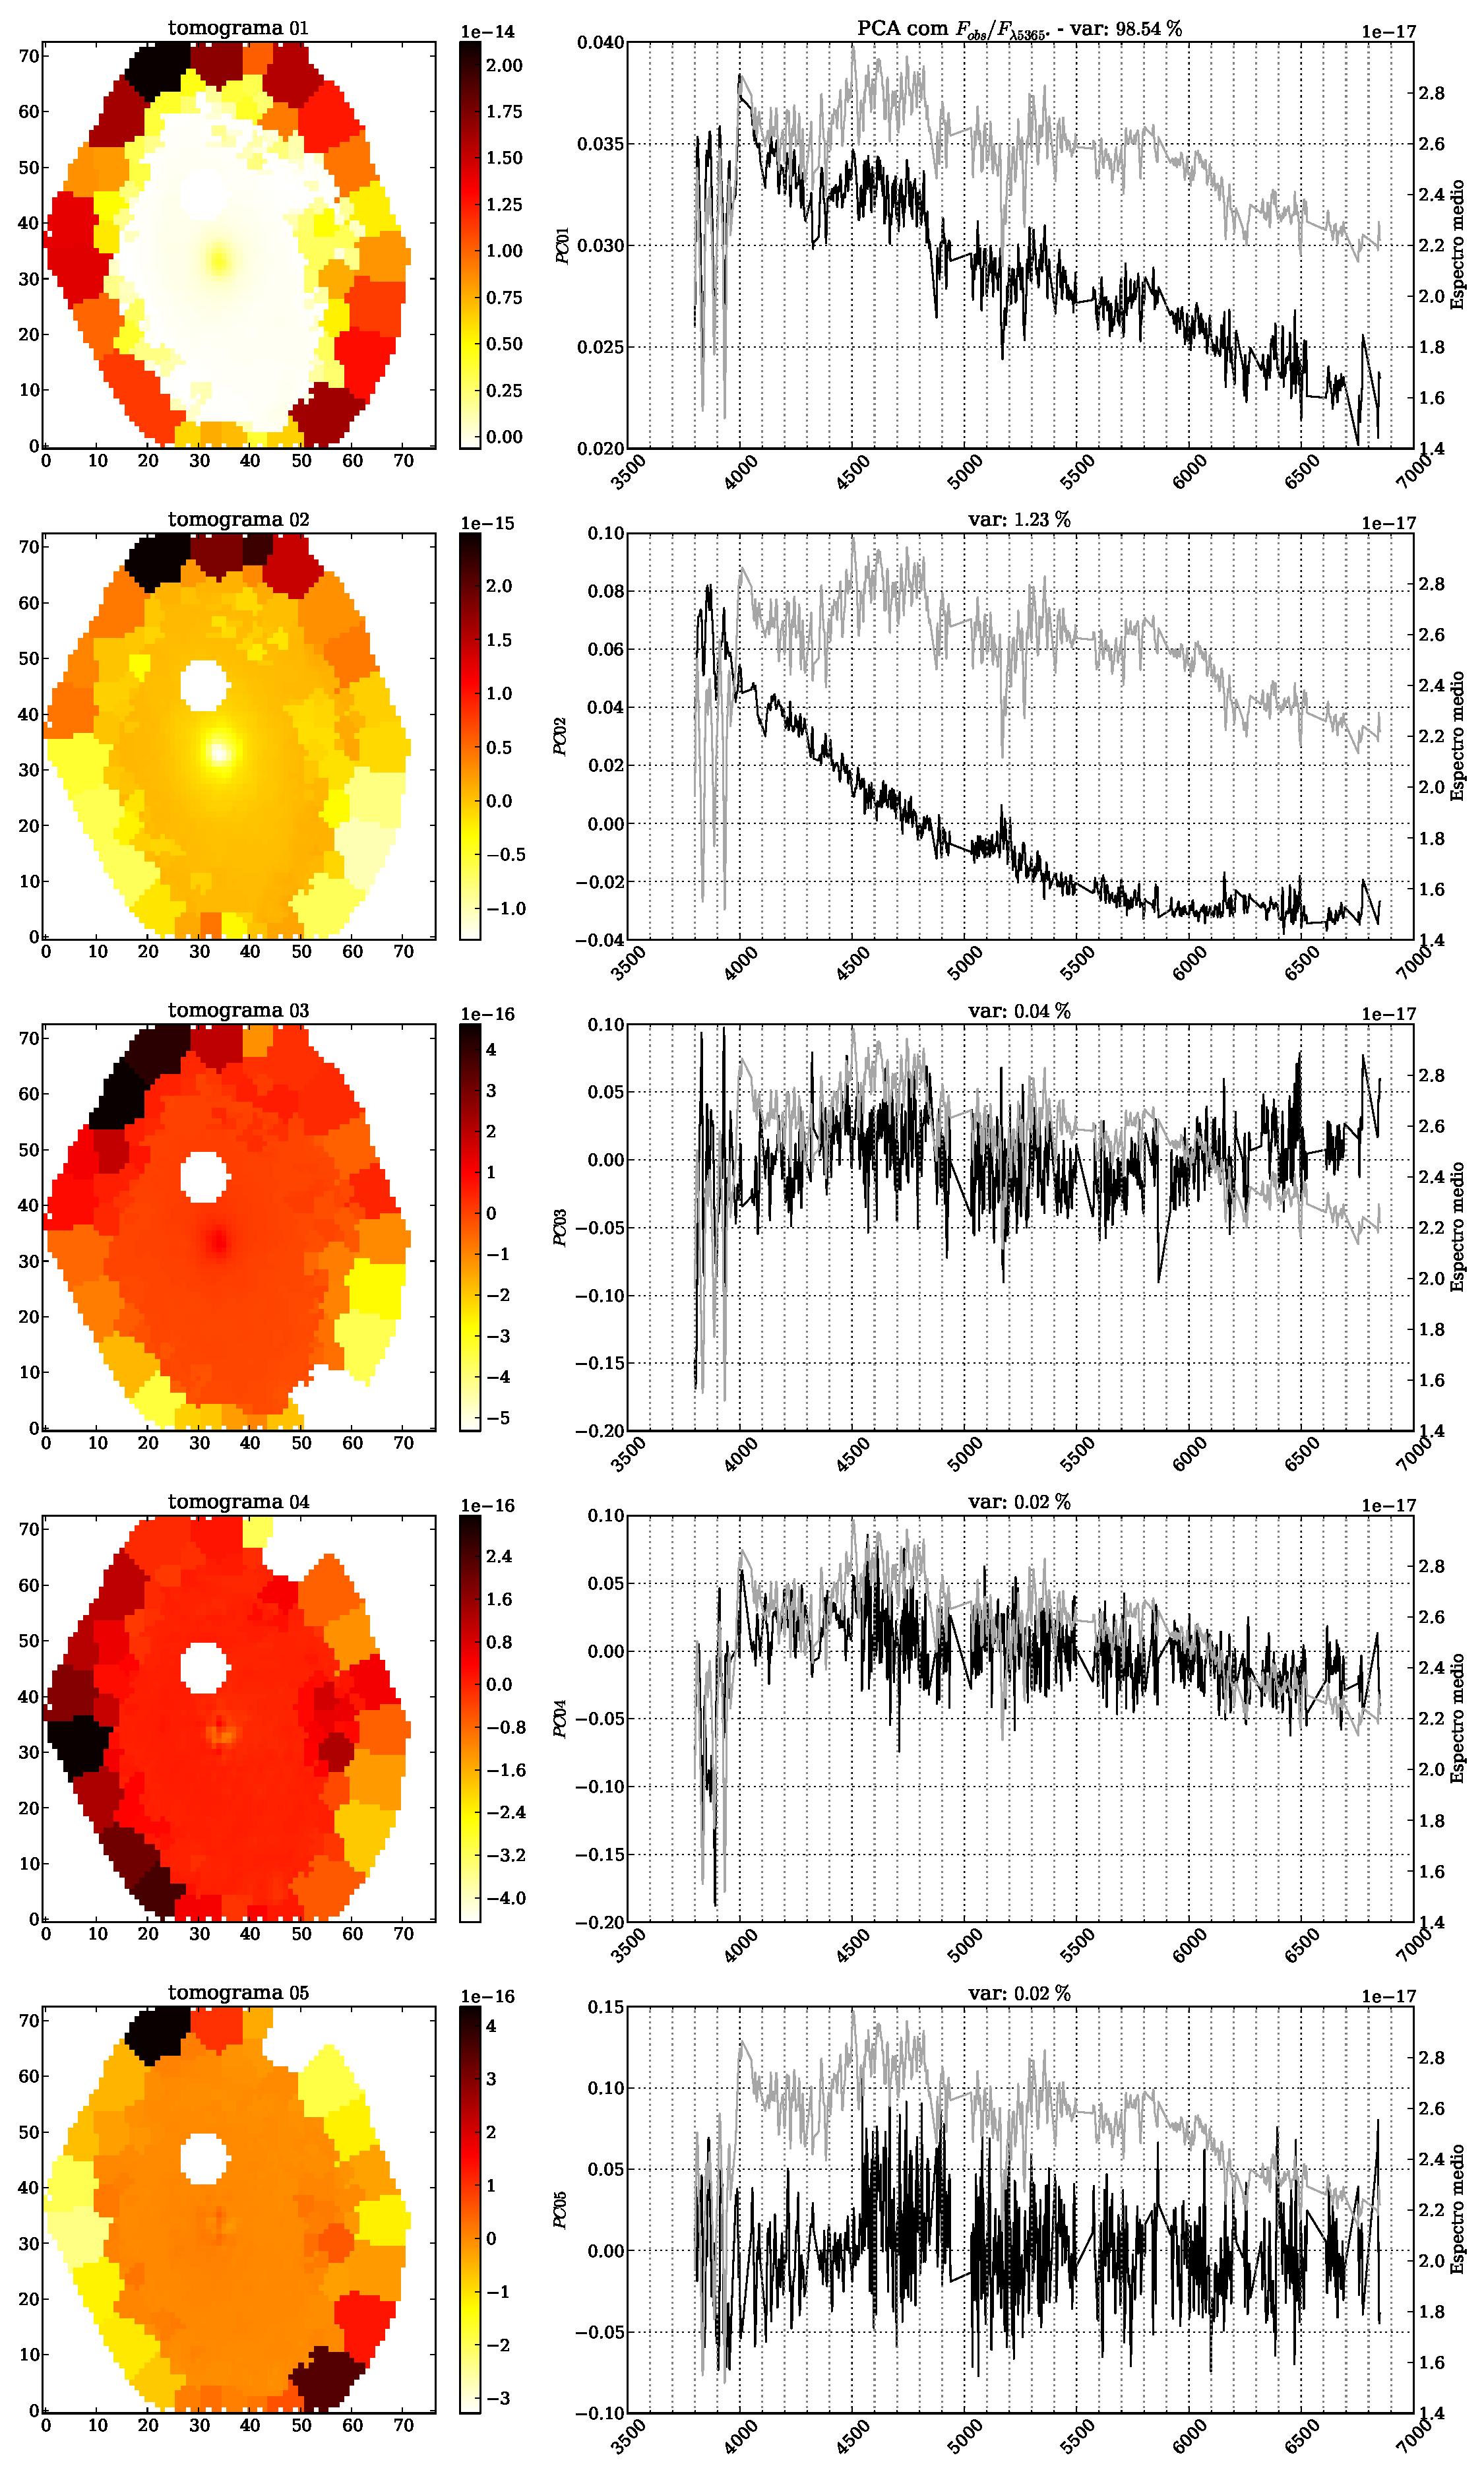
\includegraphics[width=0.8\textwidth]{figuras/K0277-tomo-obs.pdf}
    \caption[Tomogramas de 1 a 5 da gal\'axia NGC 2916 - $F_{obs}$.]
    {Cinco primeiras PCs (e seus respectivos tomogramas) resultantes da Tomografia PCA aplicado aos espectros sem
    normalização ($F_{obs}$) da galáxia NGC 2916.}
    \label{fig:K0277tomofobs}
\end{figure}

\begin{figure}
    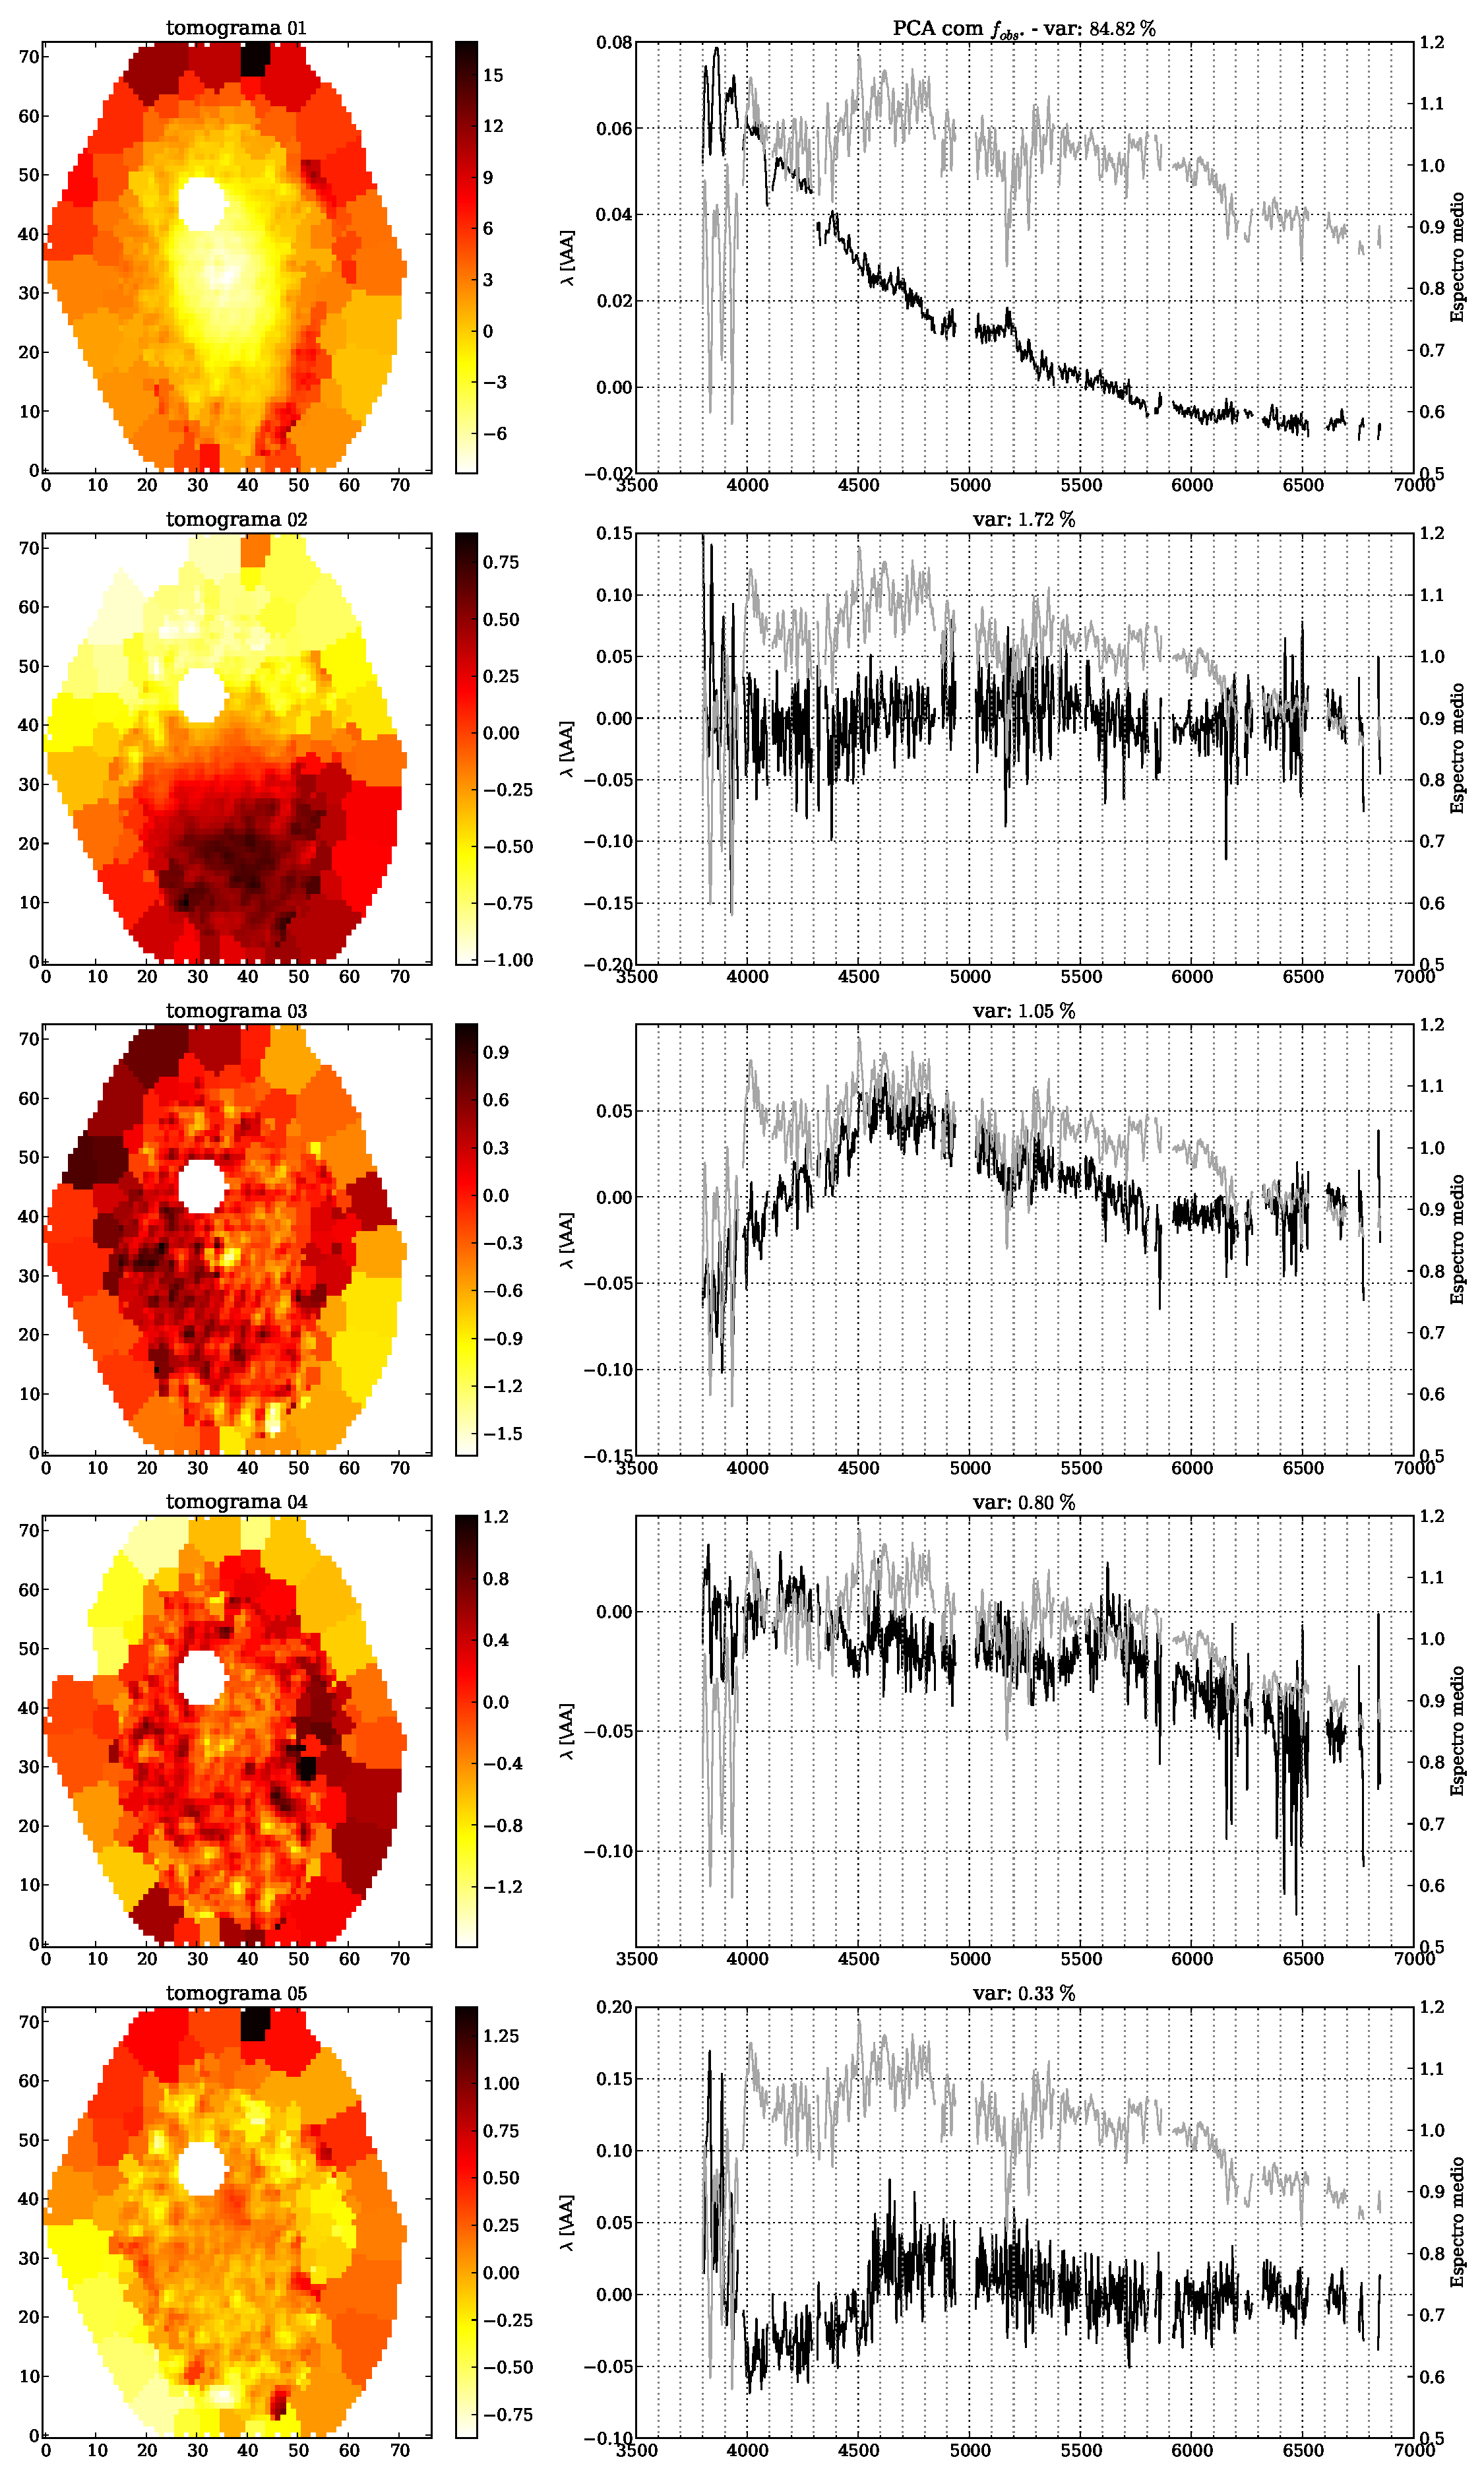
\includegraphics[width=0.8\textwidth]{figuras/K0277-tomo-obs-norm.pdf}
    \caption[Tomogramas de 1 a 5 da gal\'axia NGC 2916 - $f_{obs}$.]
    {Cinco primeiras PCs (e seus respectivos tomogramas) resultantes da Tomografia PCA aplicado aos espectros observados
    normalizados ($f_{obs}$) da galáxia NGC 2916.}
    \label{fig:K0277tomofobsnorm}
\end{figure}

\begin{figure}
    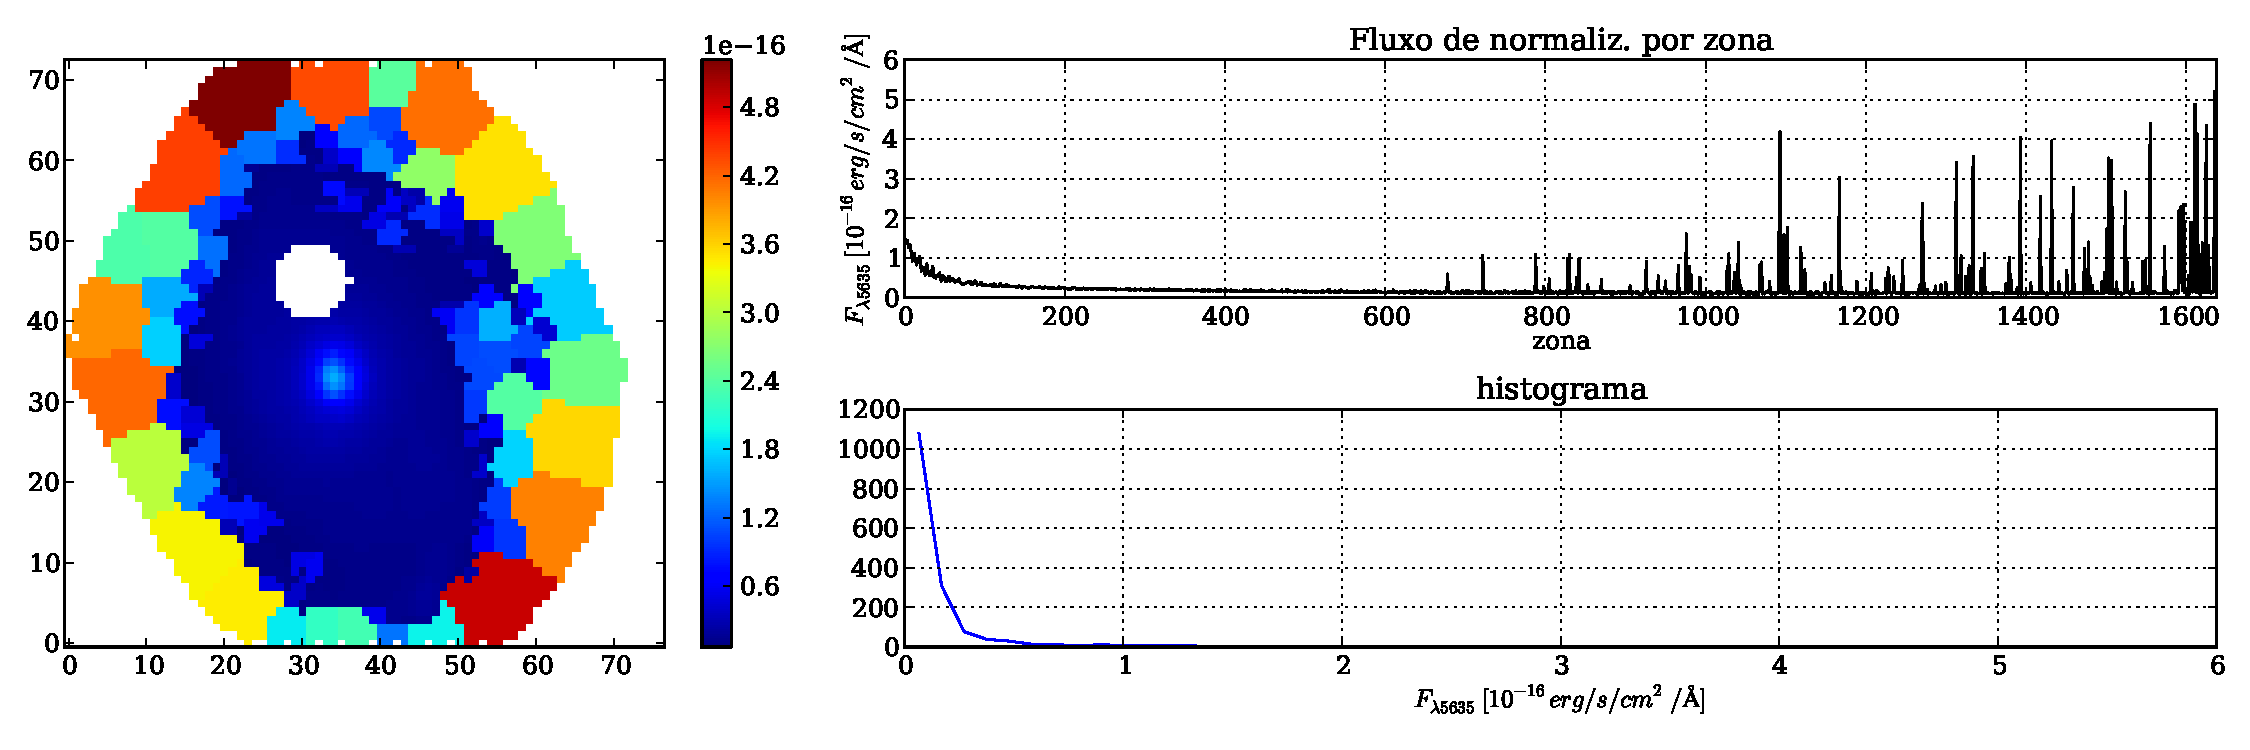
\includegraphics[width=1.\textwidth]{figuras/K0277-fobs_norm.pdf}
    \caption[Fluxos de normalização para cada zona da galáxia K0277.]
    {Fluxo usado para a normalização de cada espectro, mostrado tanto na forma de imagem (à esquerda) como em função do
    número da zona (direita).}
    \label{fig:K0277fobsnorm}
\end{figure}

\section{PCA dos espectros sintéticos}
\label{sec:PCAaplic:OBSxSYN}

Na seção anterior realizamos a PCA no cubo de espectros observados de CALIFA 277. Com o resultado da síntese de
populações estelares já organizado com o pipeline \pycasso podemos aplicar a mesma tecnica aos espectros sintéticos
gerados pelo \starlight.

A grande diferença é que nos espectros sintéticos estão contidas apenas as informações sobre populações
estelares\footnote{Efeitos de extinção/avermelhamento e cinemática também são incluidos no processo de síntese
\citep{CidFernandes2005}}. Como os espectros sintéticos não possuem as assinaturas dos equipamentos observacionais, dos
processos para subtração do céu, ruídos e afins, quando submetidas à técnica de PCA esperamos que as informações mais
relevantes se condensem em menos PCs. Comparando os dois {\em scree tests} na Figura \ref{fig:K0277scree} vemos que para
o caso com os espectros sintéticos a curva converge mais rápidamente ao zero de variância, mostrando que, como esperado,
temos as informações mais compactadas nas primeiras PCs quando comparadas ao caso com os espectros observados.
Observando o caso sem normalização, plotado no gráfico com linha pontilhada, vemos que o efeito causado pelo fator de
escala (PC1) diminui a ``importância'' (i.e., variância) das demais PCs.

\begin{figure}
    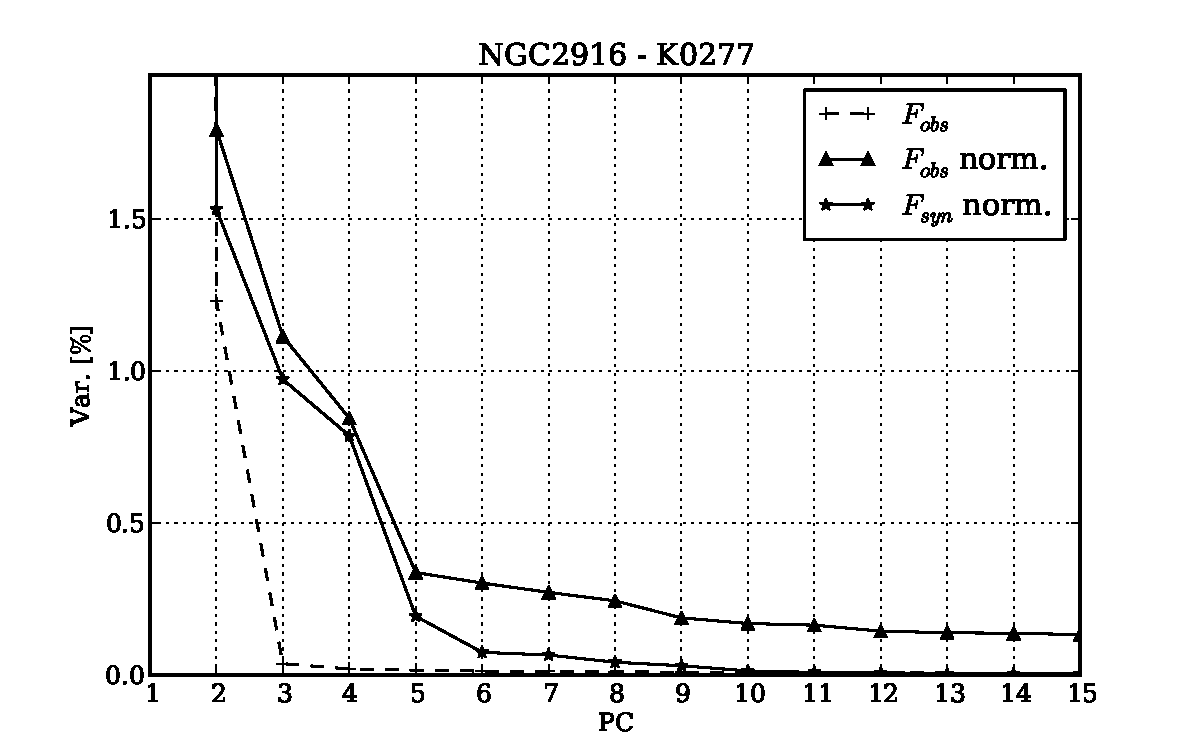
\includegraphics[width=1.\textwidth]{figuras/K0277-screetest.pdf}
    \caption[Scree test comparativo entre 3 PCAs.]
    {Scree test para 3 PCAs da galáxia NGC 2916 (CALIFA 277). Com marcações de triângulos vemos as PCs resultantes
    da PCA com os espectros observados normalizados ($f_{obs}$). As variâncias das PCs marcadas com estrela
    representam a PCA com os espectros sintéticos normalizados ($f_{syn}$). Para comparação plotamos as PCs do
    caso sem normalização ($F_{obs}$) usando linha pontilhada.}
    \label{fig:K0277scree}
\end{figure}

As cinco primeiras PCs e seus tomogramas provenientes do cubo com os fluxos sintéticos normalizados ($f_{syn}$) da
galáxia NGC 2916 aparecem na Figura \ref{fig:K0277tomofsynnorm}. Comparando com seu correspondente observacional na Figura
\ref{fig:K0277tomofobsnorm}, vemos que os resultados para os espectros sintéticos parecem ser mais ``limpos'', pois não
existem ruídos. Como são espectros gerados a partir de uma base teórica para diferentes idades e metalicidades de
populações estelares, não possuem nenhuma assinatura instrumental. Por esse fato acabamos descobrindo uma assinatura
presente em quase todas as componentes geradas pelo PCA usando os dados observados. Como comentamos no Capítulo
\ref{sec:CALePyC:Apresent} utilizamos o cubo de dados COMBO, gerado a partir da união do V500 com o V1200. Como os
espectros V1200 possuem espectros com maior resolução do que os do V500 (V1200 - FWHM $\sim 2.3$ \AA; V500 - FWHM $\sim
6$ \AA), o processo de criação do COMBO deixa vestígios. Para essa galáxia, a junção entre os dois cubos (V500 e V1200)
para a formação do COMBO acontece exatamente nesse intervalo de comprimento de onda ($\sim 4550$ \AA). O quinto
autoespectro da Figura \ref{fig:K0277tomofobsnorm} mostra um degrau entre $4500$ e $4600$ \AA\ o qual parece mostrar
essa diferença de comportamento entre as duas versões originais antes da formação do COMBO. Já nas componentes
sintéticas\footnote{Componentes geradas pela PCA nos cubos de espectros sintéticos.} não se vê essa mudança de
comportamento no autoespectro.

Assim como na análise dos espectros observados normalizados, os efeitos da cinemática se fazem notar já na segunda PC
dos cubos sintéticos, indicando que são fonte importante de variância. Consideramos, porém, que essa é uma variância
``descartável''. Usando novamente a ideia da galáxia hipotética com apenas uma população estelar, imagine agora que elas
estão distribuídas uniformemente, mas estão em rotação com a galáxia. Como anteriormente, o espectro de todos os píxels
será igual, mas agora terá deslocamentos em $\lambda$. Esses efeitos cinemáticos não estão nos trazendo informação
alguma para o estudo das populações estelares. Causam um grande desperdício de variâncias, sempre aparecendo nas
primeiras PCs. Uma manipulação através do vetor de população\footnote{O vetor de populações diz o quanto de cada
população estelar da base entra na receita para construir o espectro sintético.} criado pela síntese, juntamente com os
espectros da base, pode nos ajudar a criar os espectros sintéticos sem nenhuma correção por cinemática e poeira de
maneira que se execute a PCA sem o desperdício de variância dessas componentes cinemáticas, mas este experimento ainda
não foi realizado. Também é importante lembrar que existem métodos mais eficazes e direcionados para a determinação de
tais propriedades cinemáticas. Nas galáxias presentes no CALIFA não poderia ser diferente, portanto os espectros
aparecem com linhas deslocadas para o azul ({\em blue-shifted}) ou para o vermelho ({\em red-shifted}) dependendo da
velocidade de rotação projetada. 

\begin{figure}
    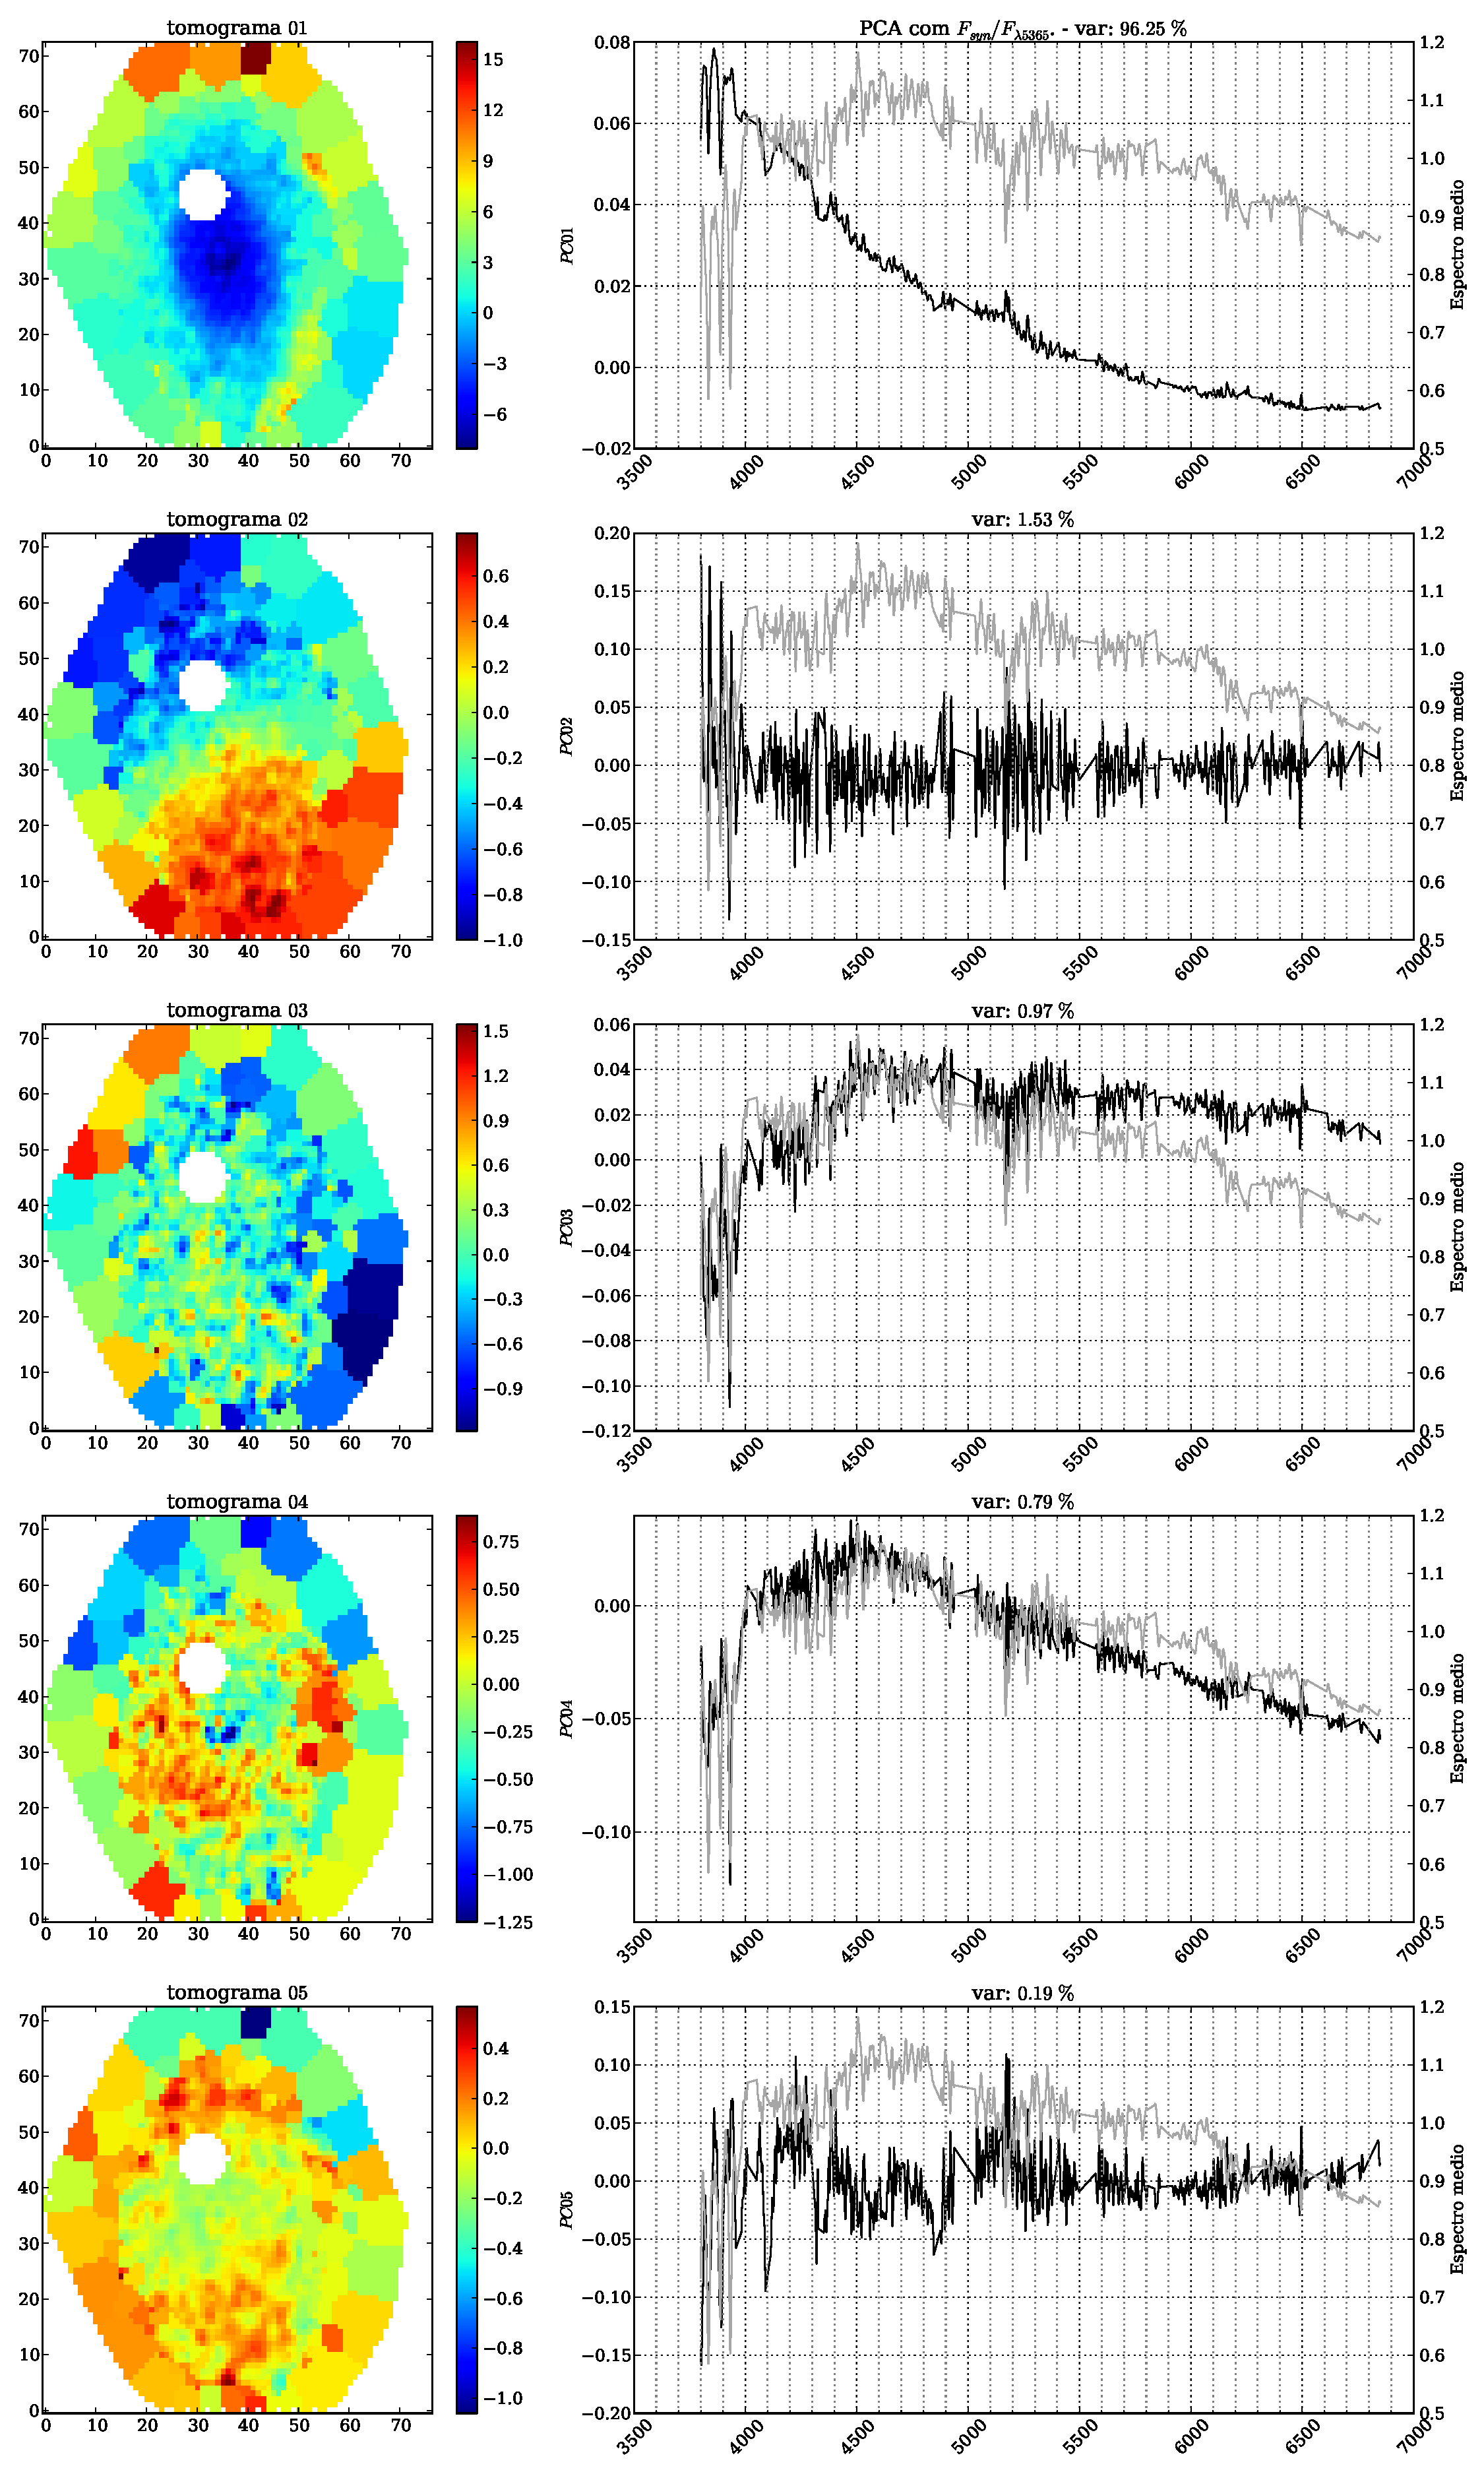
\includegraphics[width=0.8\textwidth]{figuras/K0277-tomo-syn-norm.pdf}
    \caption[Tomogramas de 1 a 5 da gal\'axia NGC 2916 - $f_{syn}$ .]
    {Cinco primeiras PCs (e seus respectivos tomogramas) resultantes da Tomografia PCA aplicado aos espectros
    sintéticos normalizados ($f_{syn}$) da galáxia NGC 2916.}
    \label{fig:K0277tomofsynnorm}
\end{figure}

%\section{PCA logarítmica}
%\label{sec:PCAaplic:PCAlog}
%
%Um outro experimento que realizamos foi calcular o PCA sobre os logarítmos dos espectros.  Essa variante da analise
%pode ser vista como uma mera curiosidade matematica, uma experiencia para ver o que se obtem. No entanto, ela foi inspirada
%em um motivo físico: É razoavel esperar que utilizando o log possamos ressaltar efeitos devidos a gradientes de poeira,
%já que a extincao que atua de forma multiplicativa sobre os espectros.
%
%Para entender melhor voltemos ao caso hipotetico de uma galaxia na qual as populacoes estelares sao iguais em todas
%partes e na qual as estrelas estao todas paradas, de modo que nao ha deslocamentos nnem modulacoes em $\lambda$ devido
%a efeitos de cinematica. Neste caso, as variacoes de $\textbfF{}_{z \lambda}$ entre as diferentes zonas vem tanto do
%efeito de amplitude (brilho superficial) já estudado como de diferencas na profudindade optica da poeira $\tau_{z
%\lambda}$. O efeito global de amplitude pode ser removido com nosso esquema de normalizacao, mas as variacoes de
%$\tau_{z \lambda}$ de zona a zona afetam a forma do espectro observado.
%
%O efeito da poeira é atenuar um fluxo intrinseco $F^i$ por um fato $e^{-\tau}$, produzindo um fluxo observado
%(transmitido) $F^o$. Escrevendo $F^o = F^i e^{-\tau}$ para um certo $\lambda$ e normalizando-o pelo comprimento de onda
%de normalizacao $\lambda_N$ obtemos
%
%\begin{equation}
%\frac{\textbfF^o_{z \lambda} }{\textbfF^o_{z \lambda_N} } =
% \frac{\textbf{F}^i_{z \lambda}  }{\textbf{F}^i_{z \lambda_N} } 
% \frac{ e^{-\tau_{z \lambda}} }{ e^{-\tau_{z \lambda_N}}}
%\end{equation}
%
%Denotando os espectros normalizados por $O_\lambda$ e assumindo que a lei de extincao é a mesma em todas zonas
%
%\begin{equation}
%\textbf{O}^o_{z \lambda} = \textbf{O}^i_{z \lambda}
% e^{-\tau_{z V} (q_\lambda - q_{\lambda_N})}
%\end{equation}
%
%\noindent onde $q_\lambda \equiv \tau_\lambda / \tau_V$ regula o grau de avermelhamento. Tirando o ln
%
%\begin{equation}
%\ln \textbf{O}^o_{z \lambda} = \ln \textbf{O}^i_{z \lambda}
% -\tau_{z V} (q_\lambda - q_{\lambda_N})
%\end{equation}
%
%Se $\textbf{O}^i_{z \lambda}$ é igual para todas zonas, como é o caso em nossa galáxia hipotética, fica claro que toda
%variancia em $\ln \textbf{O}^o_{z \lambda}$ estará associada a variancia de $\tau_{z V}$ de zona-a-zona, e a tomografia
%PCA mapeará essa variancia. Sem as operacoes de normalizacao e logaritmo, esse efeito apareceria misturado com outros.
%
%CALIFA 277, a galáxia que temos usado como exemplo ao longo desse capitulo, contem pouca poeira, nao sendo portanto um
%bom caso para aplicacao dessa variante. Exemplificaremos os resultados da PCA logaritimica no capitulo 5 ao estudarmos
%os sistemas em fusao ({\em mergers}) Arp 220 e NGC ????, ricos em poeira.

\section{Comparando as PCs com o \STARLIGHT: engenharia reversa}
\label{sec:PCAaplic:EngRev}

Descobrir o sentido físico de cada PC não é tarefa fácil. Como comentamos anteriormente, o PCA te dá a resposta, mas
você geralmente não sabe qual a pergunta. Uma forma de buscar sentido físico nas componentes é analisar as correlações
com propriedades físicas da galáxia.

Com o resultado da síntese de populações estelares obtido pelo \starlight e organizado pelo \pycasso fica simples
correlacionarmos os dados na base gerada pela PCA. Nas Figuras \ref{fig:K0277correfobsnorm} e
\ref{fig:K0277correfsynorm} vemos as correlações entre algumas propriedades físicas (\meanL{\log\ t}, $\log\ \meanL{Z}$,
$A_V$, $v_{\star}$, $\sigma_{\star}$) e o peso de cada PC por zona (tomograma versus propriedade física) para CALIFA
277. O número presente em cada gráfico é o coeficiente de correlação por {\em rank} de Spearman. Escolhemos o
coeficiente de Spearman pois este é aparamétrico e, ao contrário do coeficiente de Pearson, não pressupõe nenhuma
relação linear. Em cada coluna temos uma quantidade física e na última coluna temos o autovetor representado por aqueles
pontos.

Tanto para os dados observados quanto sintéticos vemos que a primeira PC representa basicamente um fator de idade.
Possui correlação também com a metalicidade. A segunda PC também em ambos os casos representa uma forte correlação com a
velocidade estelar, refletindo a curva de rotação da galáxia. A terceira PC com os dados observados parece ser um bom
sensor para o padrão global de extinção ($A_V$). Essa PC parece se dissolver em duas no caso do espectro sintético (PC3
e 4). As PC4 e PC5 no caso observado não parecem ter correlação com nenhum desses parâmetros físicos comparados, salvo
pequenas correlações com $A_V$ e $v_\star$ na PC5. Essa última, para o caso sintético, parece estar correlacionada com
$A_V$ também, mas de forma mais fraca. Também possui um padrão de correlação com $v_\star$. Por fim, a PC6 no caso
observado parece ter uma mistura de idade, metalicidade, extinção e com a dispersão de velocidades. Para o caso
sintético existe uma correlação com a metalicidade e a dispersão de velocidades. Um padrão de rotação também aparece mas
com um coeficiente de Spearman baixo.

Outra forma de se observar essas correlações é graficando os dados nos eixos das PCs, colorindo os pontos por
determinado parâmetro físico. No Apêndice estarão todos os gráficos com todos os parâmetros físicos. Como exemplo aqui
deixamos as Figuras \ref{fig:K0277correfobsnormPCvsPC:AV} e \ref{fig:K0277correfsynnormPCvsPC:AV} que mostram
as PCs para o caso observado e sintético, coloridos pelo $A_V$.

\begin{figure}
    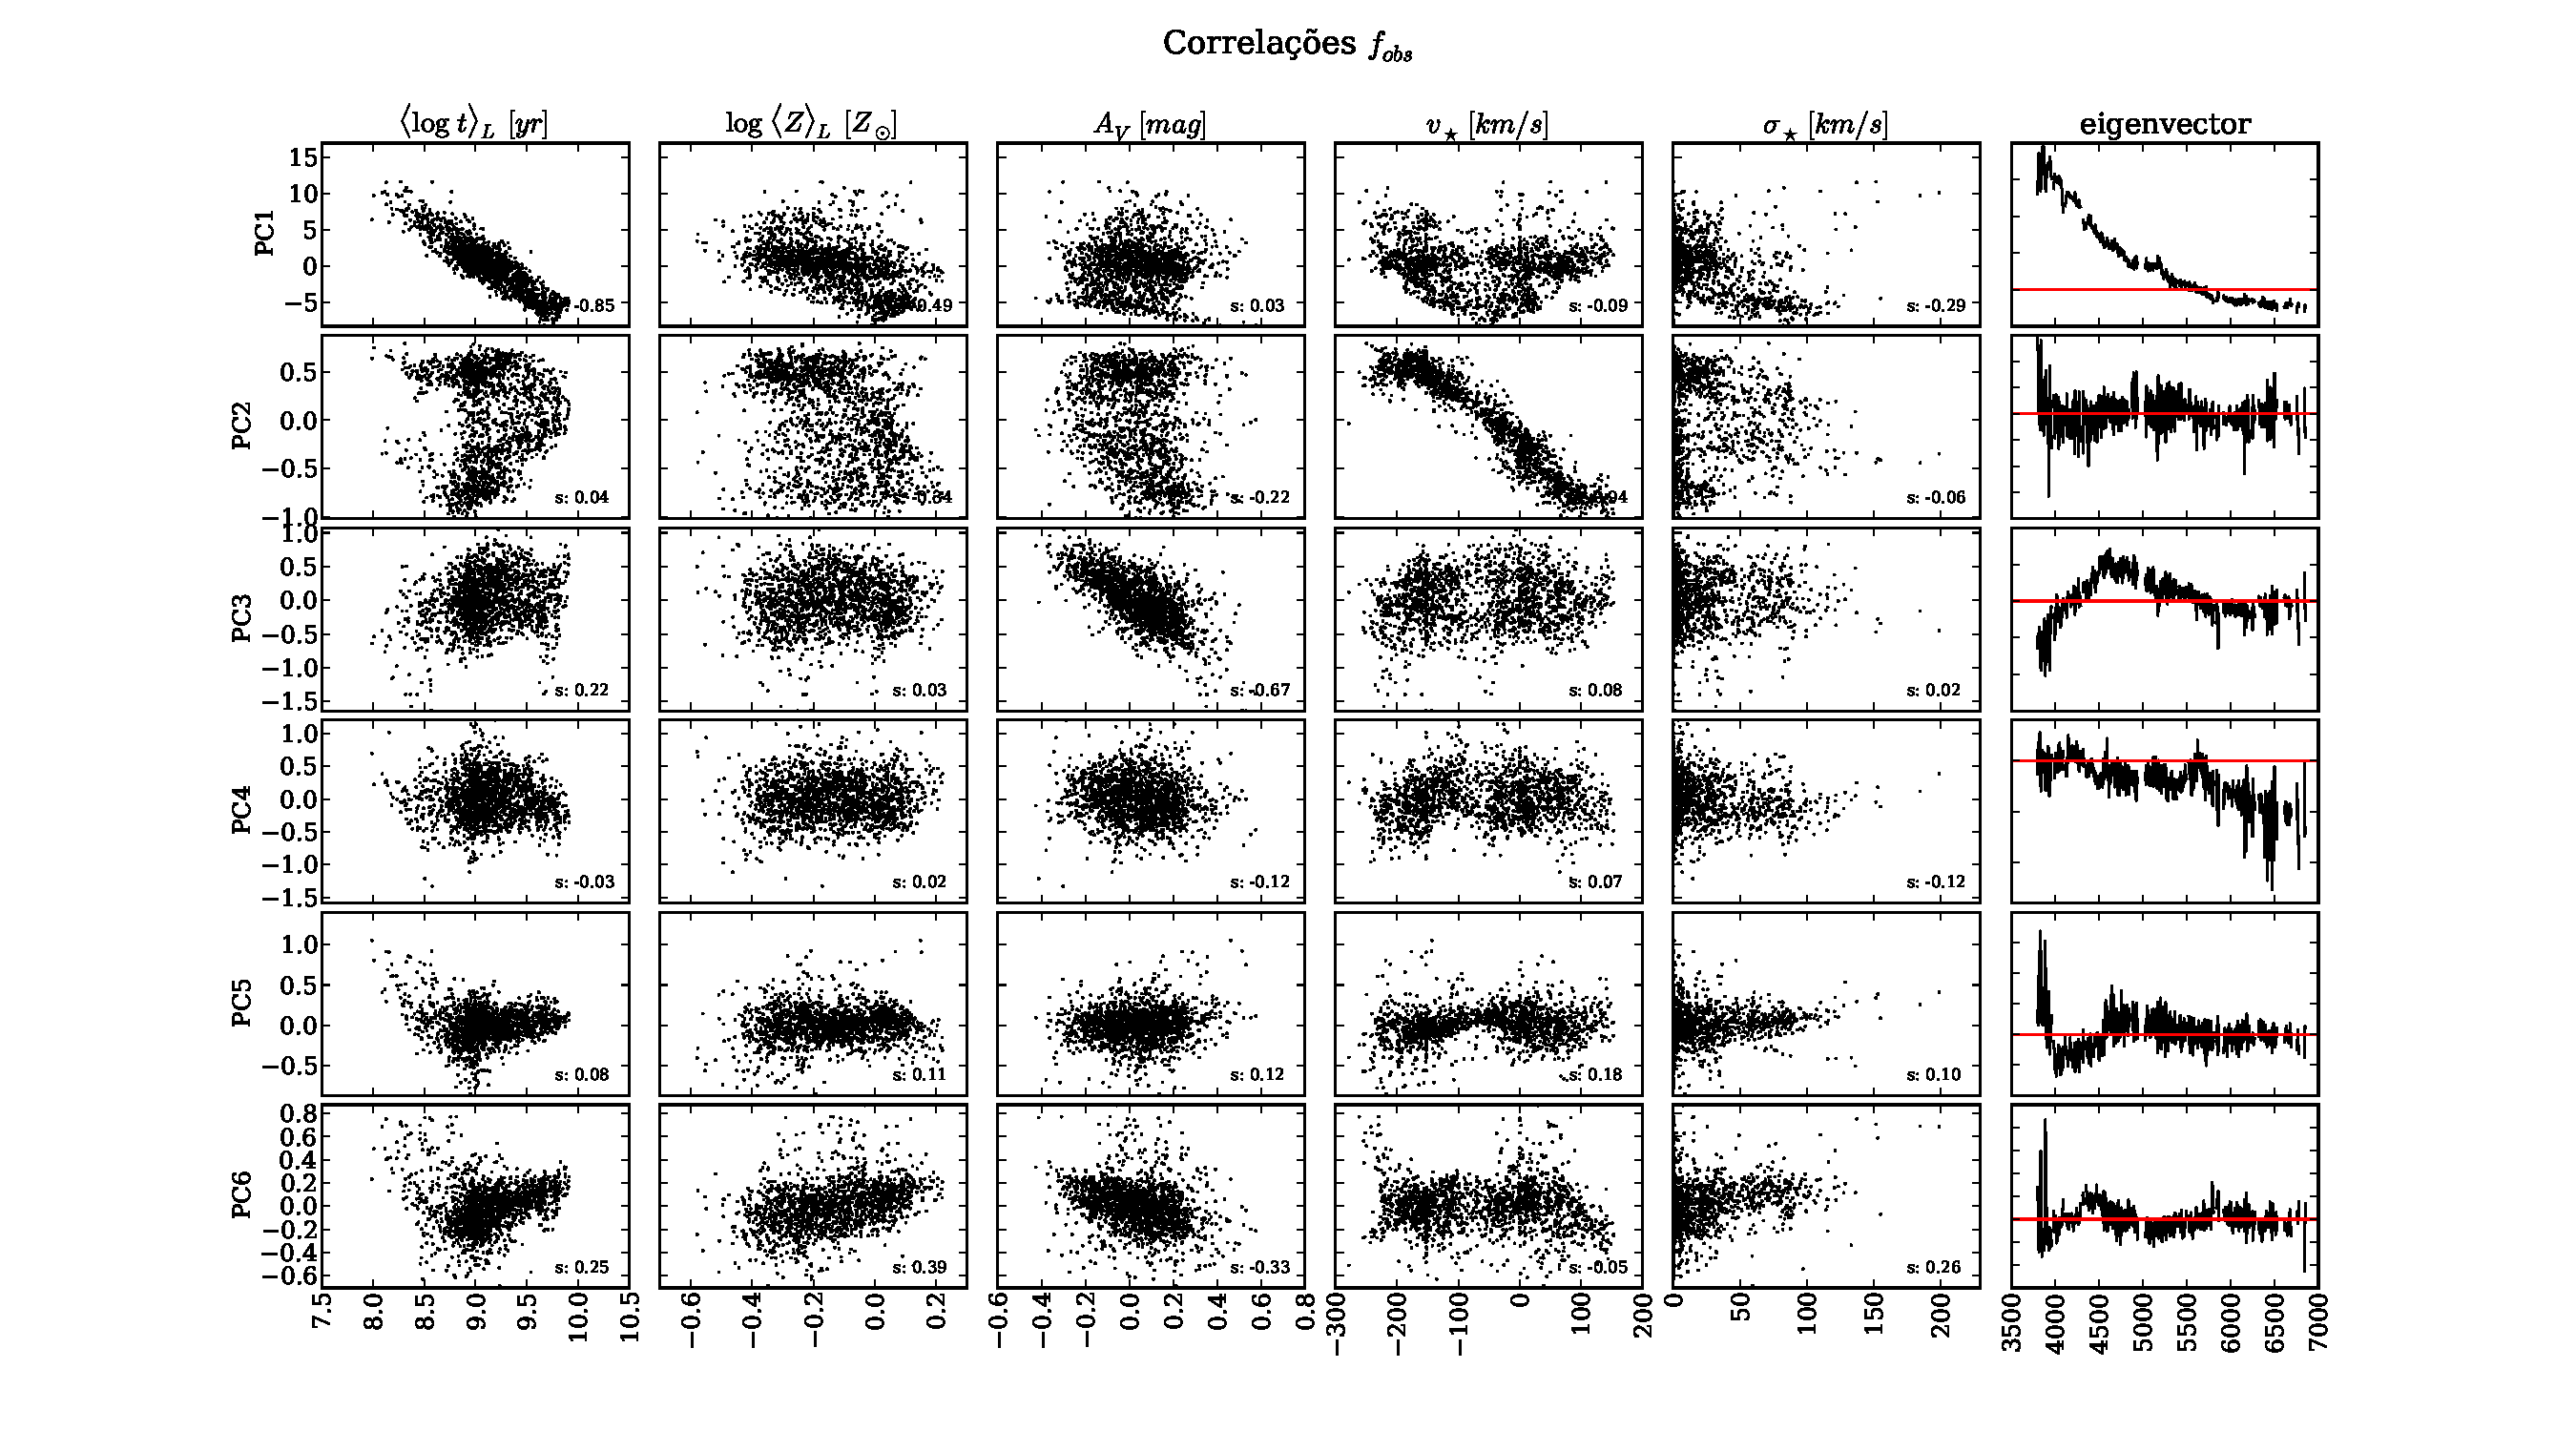
\includegraphics[width=1.2\textwidth,angle=-90]{figuras/K0277-correl-f_obs_norm-PCvsPhys.pdf}
	\caption[Correlações PCs vs. par\^ametros f\'isicos - $f_{obs}$.]
    {Correlações entre os pesos por zona das seis primeiras PCs da PCA feito para o cubo com os dados observados
    normalizados ($f_{obs}$) e cinco parâmetros físicos. Pela ordem de colunas da esquerda para direita temos
    $\meanL{\log\ t}$, $\log\ \meanL{Z}$, $A_V$, $v_{\star}$, $\sigma_{\star}$. Na última coluna temos o autoespectro para ajudar na
    visualização. A linha em vermelho no gráfico do autoespectro serve para identificar o zero. O número dentro de
    cada gráfico é o coeficiente de correlação de Spearman.}
    \label{fig:K0277correfobsnorm}
\end{figure}

\begin{figure}
    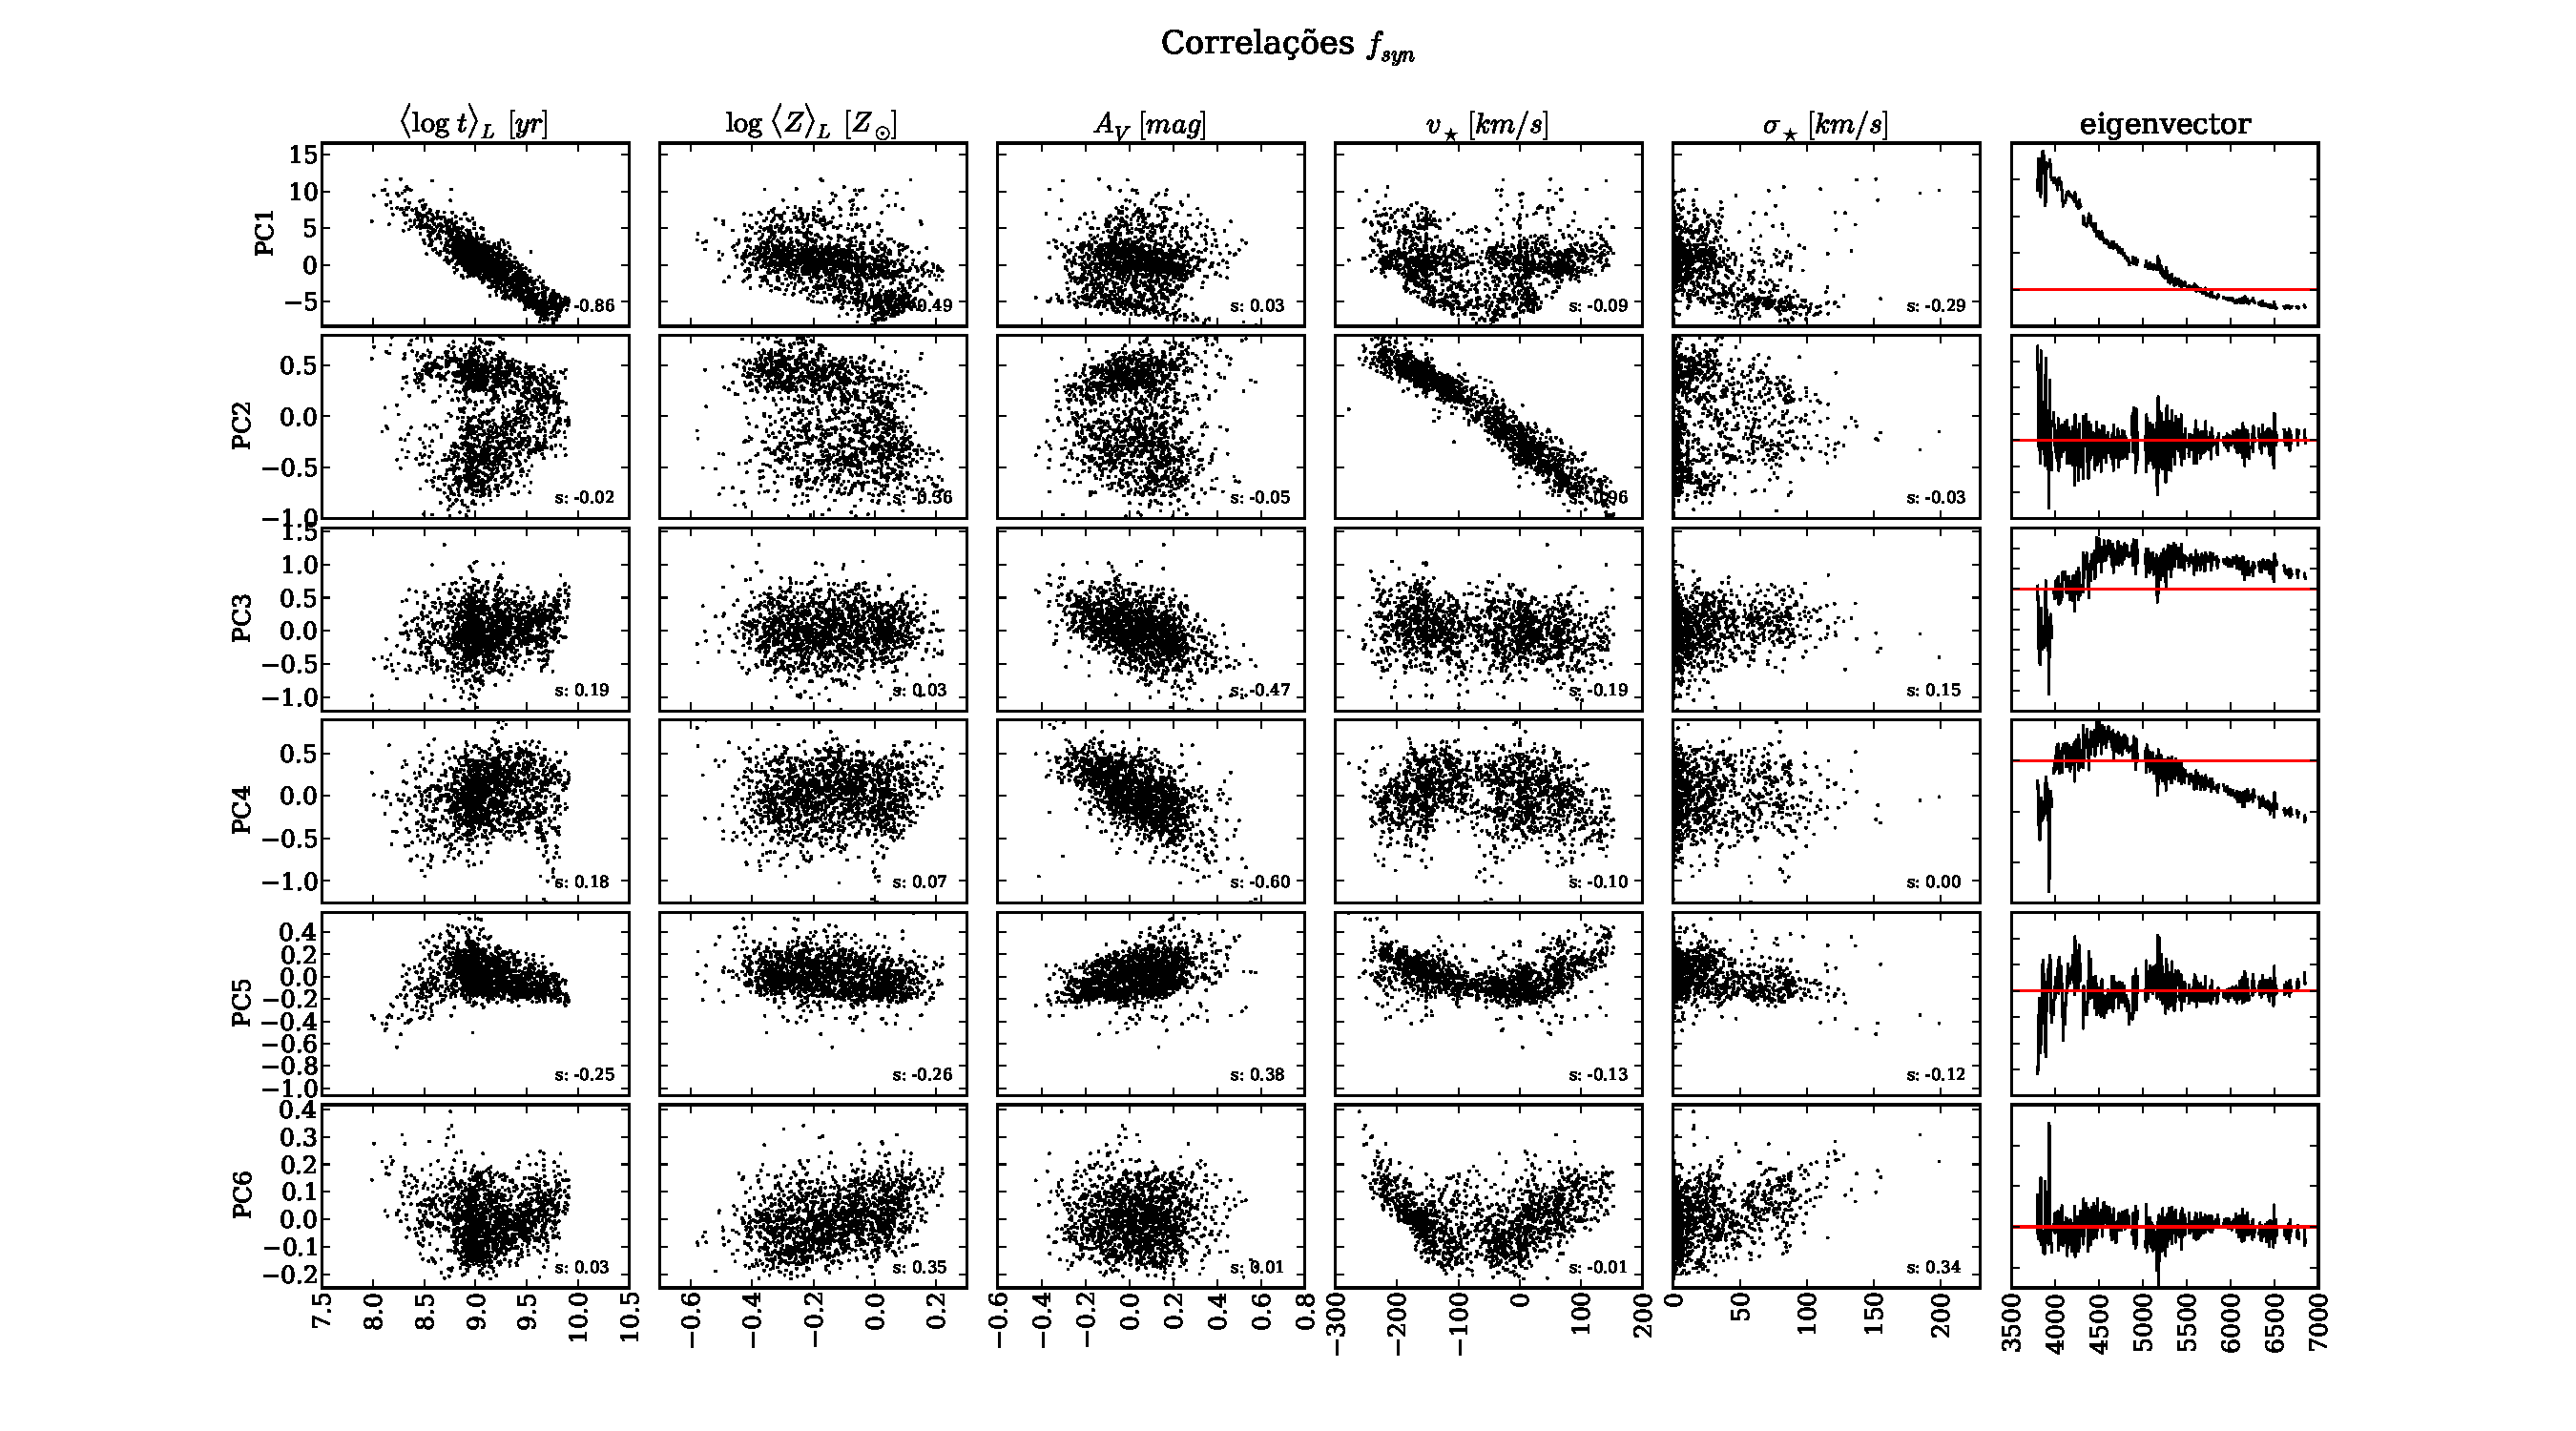
\includegraphics[width=1.2\textwidth, angle=-90]{figuras/K0277-correl-f_syn_norm-PCvsPhys.pdf}
	\caption[Correlações PCs vs. par\^ametros f\'isicos - $f_{syn}$.]
    {Correlações entre os pesos por zona das seis primeiras PCs da PCA feito para o cubo com os dados sintéticos
    normalizados ($f_{syn}$) e cinco parâmetros físicos. Pela ordem de colunas da esquerda para direita temos
    $\meanL{\log\ t}$, $\log\ \meanL{Z}$, $A_V$, $v_{\star}$, $\sigma_{\star}$. Na última coluna temos o autoespectro para ajudar na visualização.
    A linha em vermelho no gráfico do autoespectro serve para identificar o zero. O número dentro de cada gráfico é o
    coeficiente de correlação de Spearman.}
    \label{fig:K0277correfsynorm}
\end{figure}

\begin{figure}
	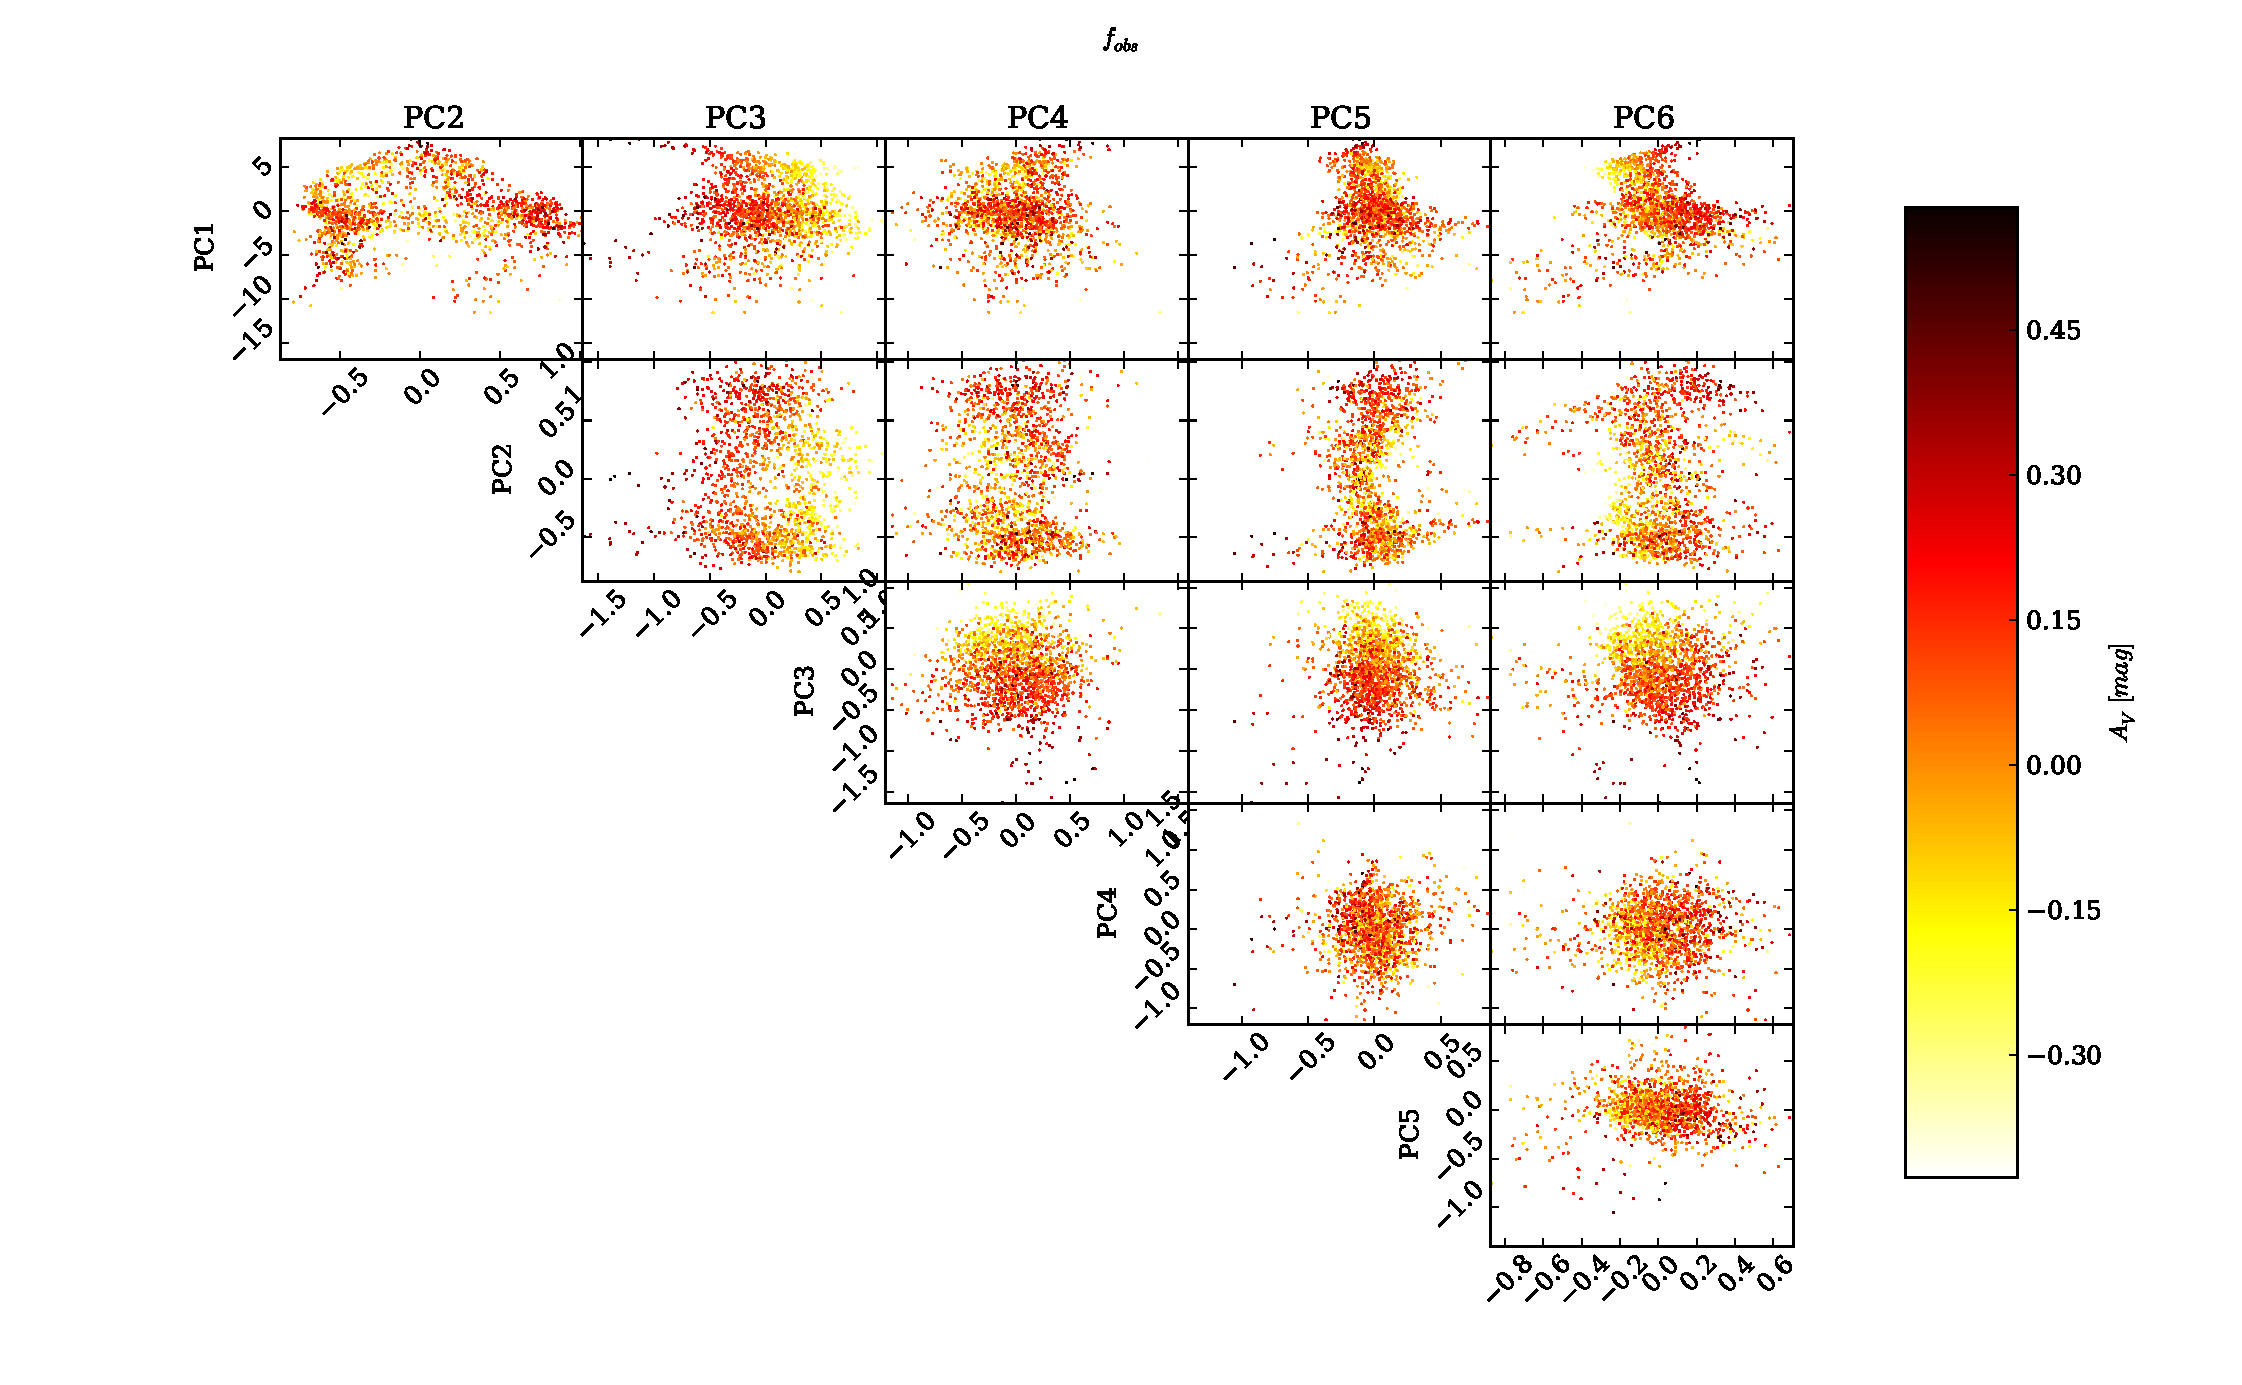
\includegraphics[width=1.3\textwidth, angle=-90]{figuras/K0277-f_obs_norm-corre_PCxPC_AV.pdf}
	\caption[Dados no espaço das PCs vs AV- $f_{obs}$.]
    {Dados das zonas no espaço das PCs ($f_{obs}$) coloridos pela extinção ($A_V$).}
    \label{fig:K0277correfobsnormPCvsPC:AV}	
\end{figure}

\begin{figure}
	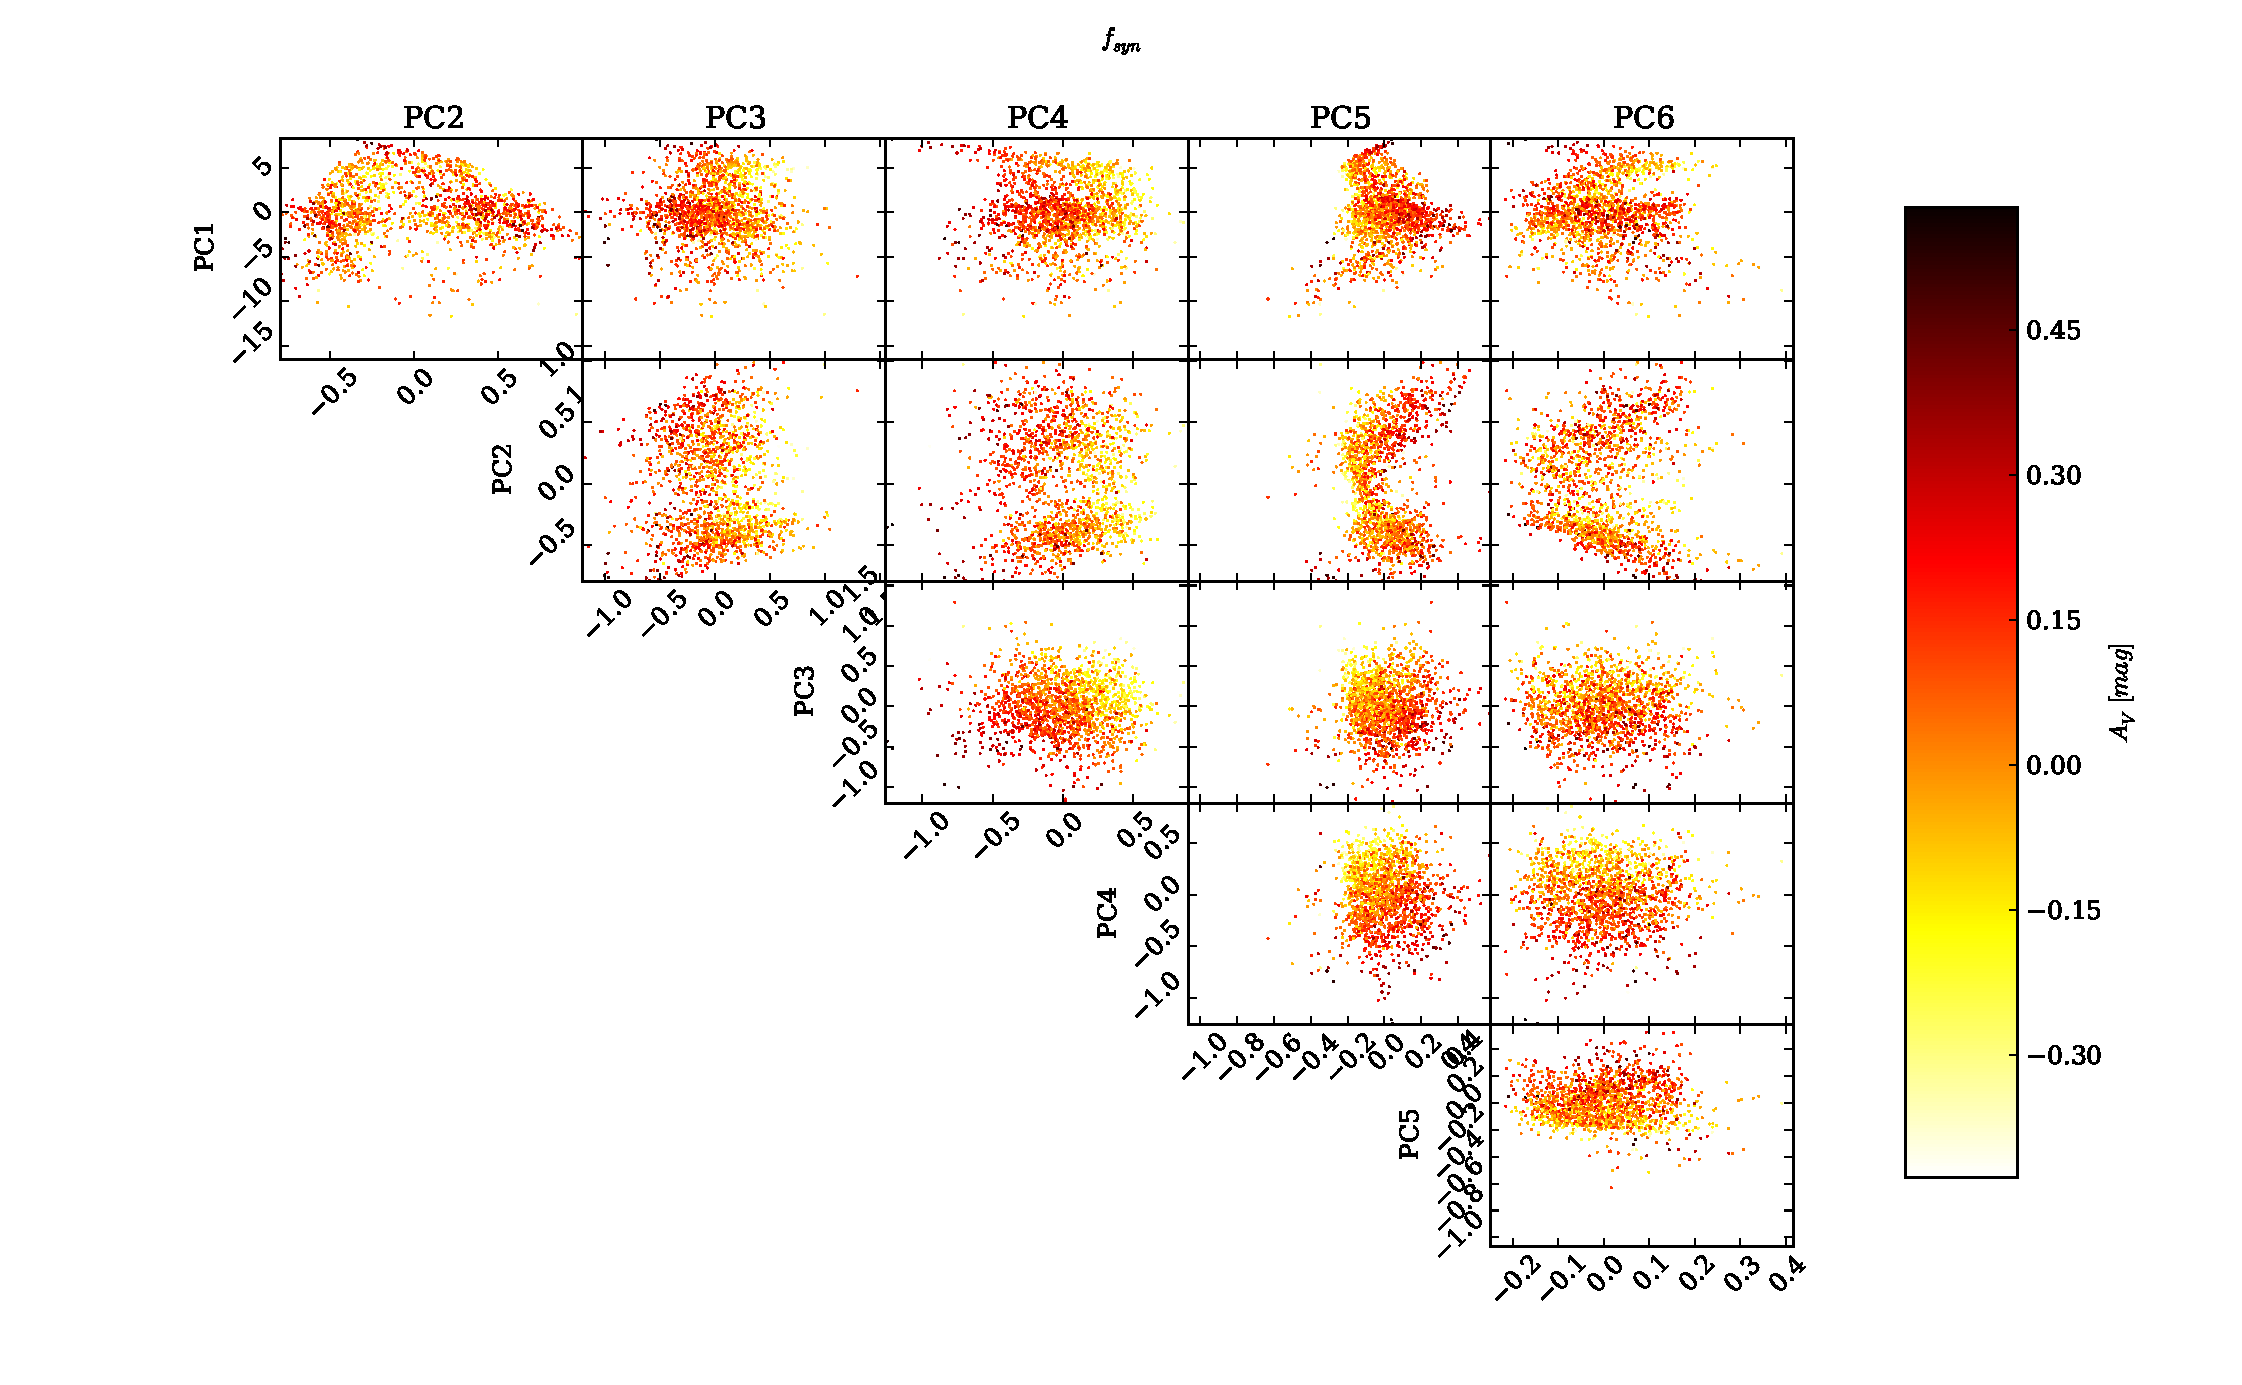
\includegraphics[width=1.3\textwidth, angle=-90]{figuras/K0277-f_syn_norm-corre_PCxPC_AV.pdf}
	\caption[Dados no espaço das PCs vs AV- $f_{syn}$.]
    {Dados das zonas no espaço das PCs ($f_{syn}$) coloridos pela extinção ($A_V$).}
    \label{fig:K0277correfsynnormPCvsPC:AV}	
\end{figure}

A Figura \ref{fig:K0277correfobs} mostra também o efeito que a falta de normalização faz com o resultado da PCA. Esse
fator de amplitude que não é removido pela normalização se concentra principalmente na primeira PC, mas ainda deixa
vestígios se misturando com as outras PCs fazendo com que haja correlação entre cada PCs e quase todos os parâmetros
físicos. Por mais esse motivo, deixaremos a PCA dos espectros não normalizados de lado no restante desse trabalho.

\begin{figure}
    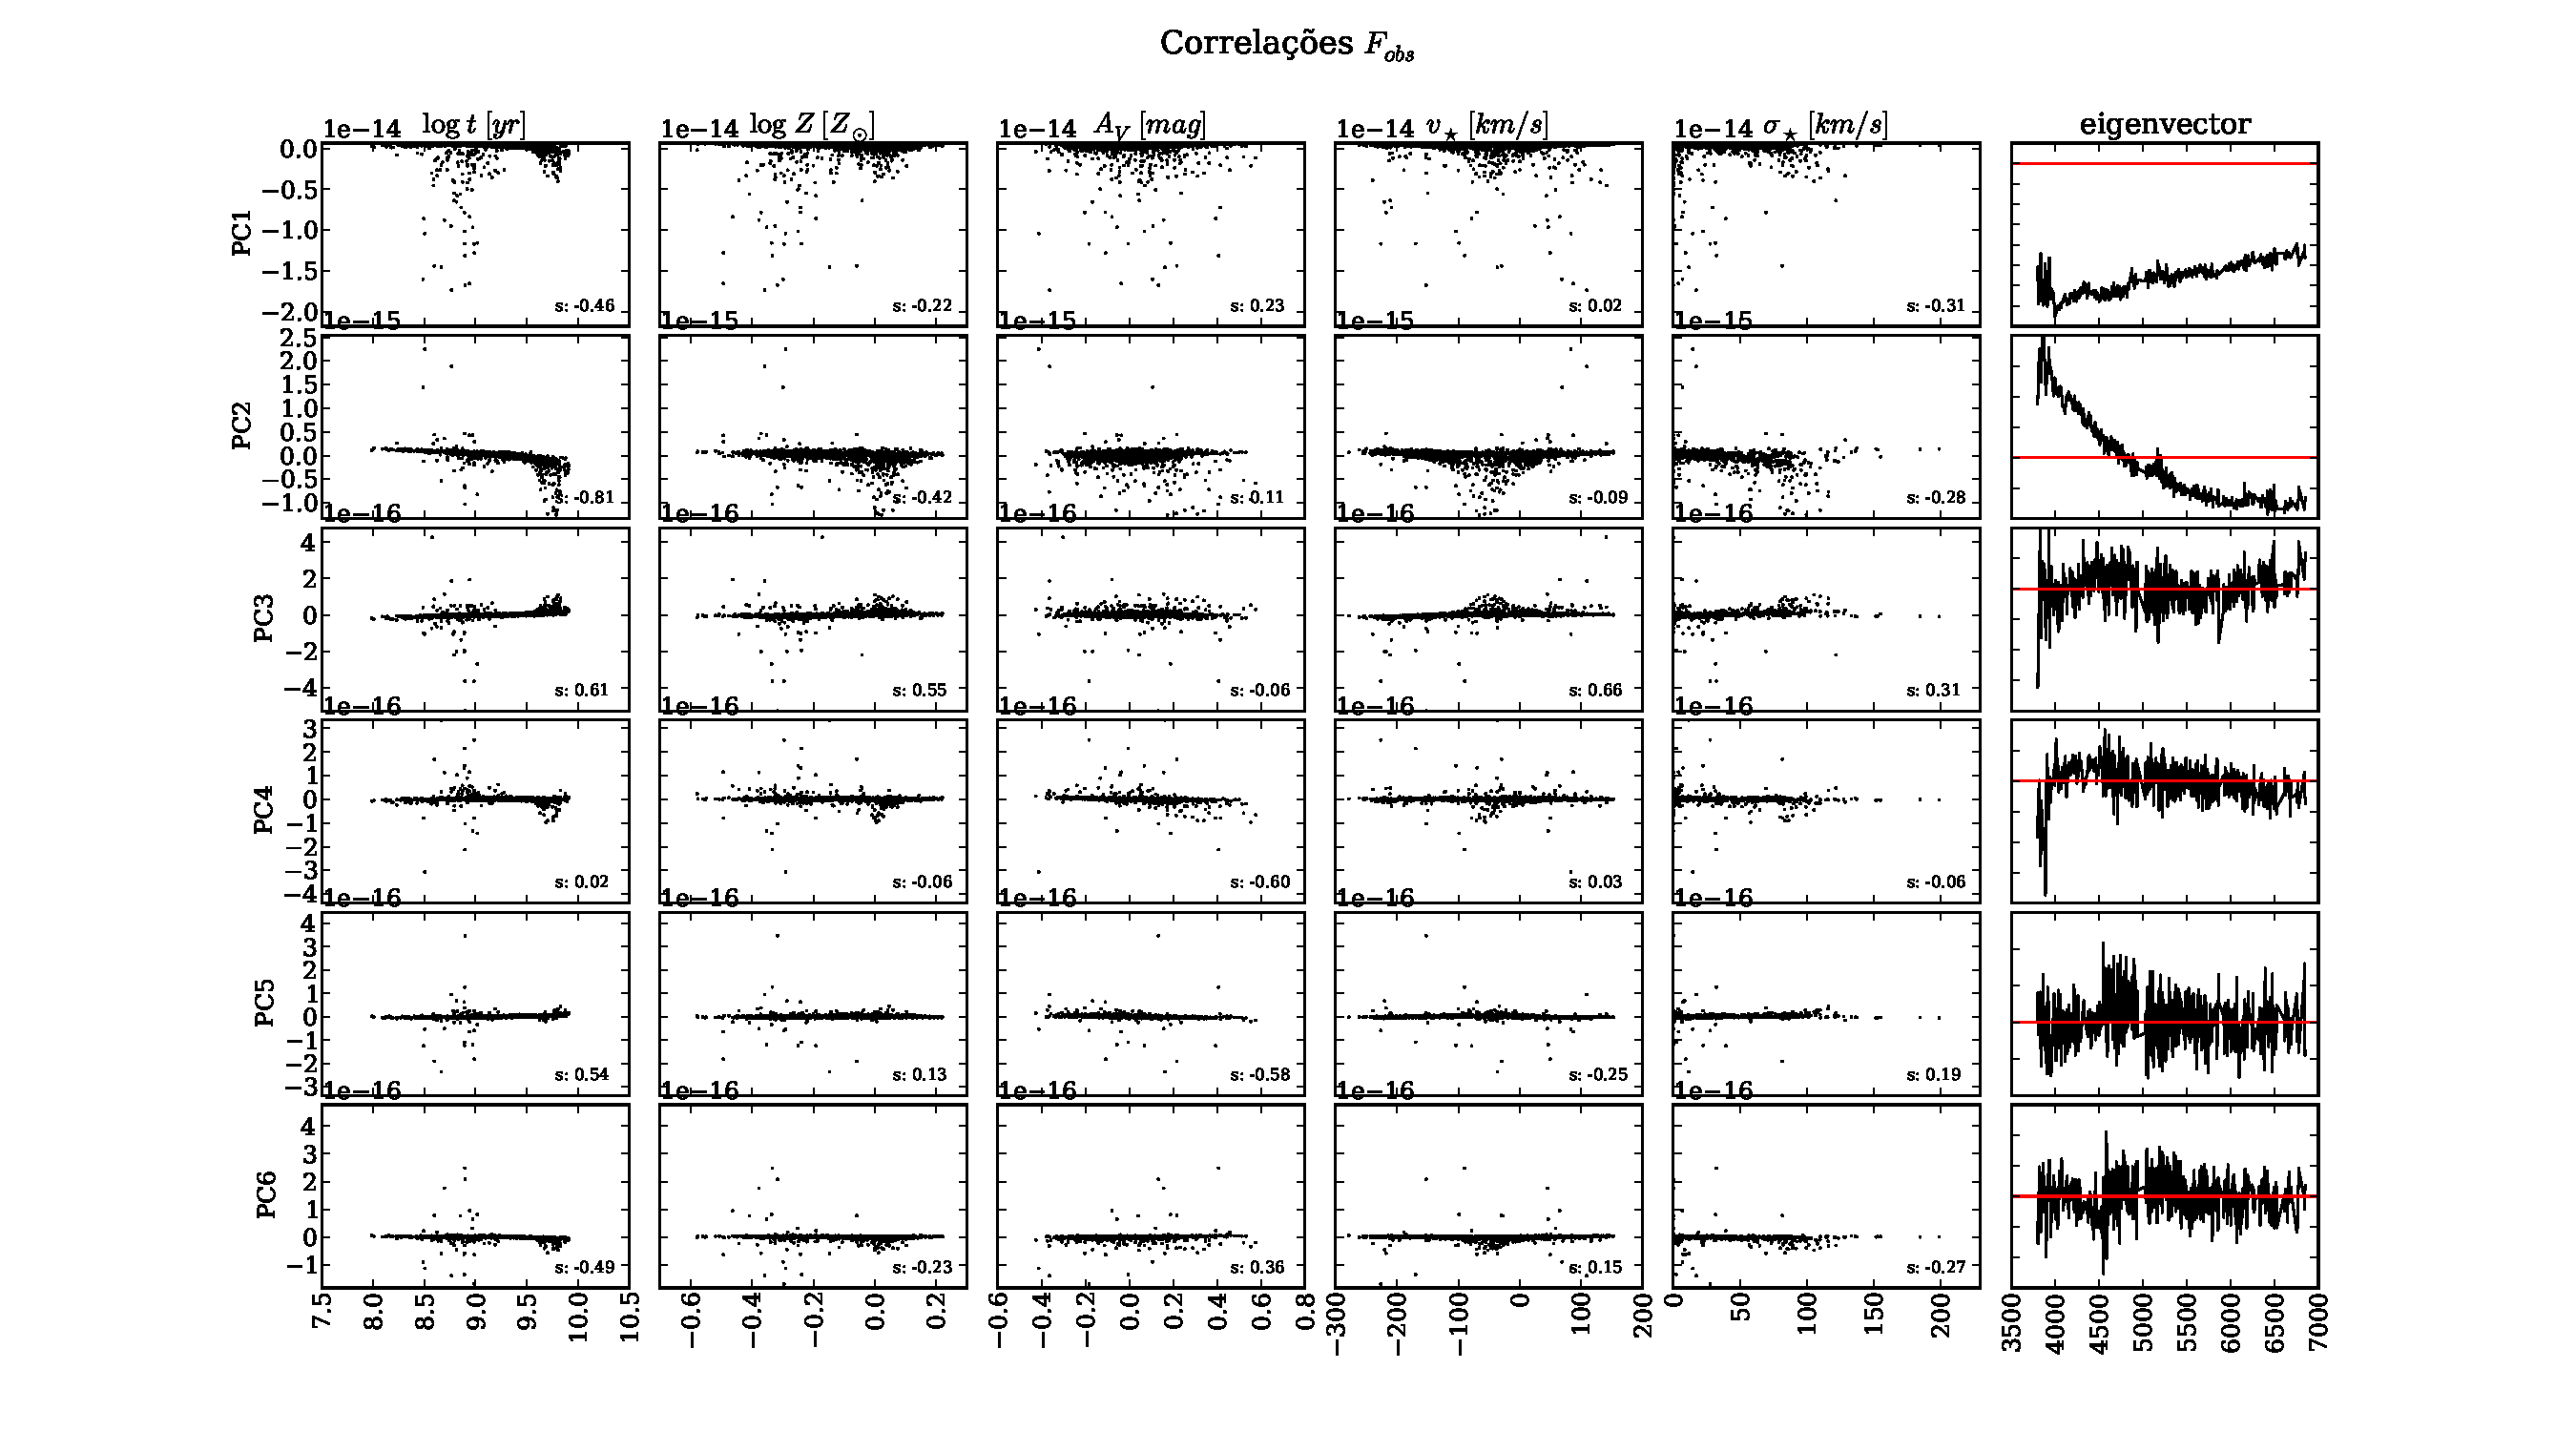
\includegraphics[width=1.2\textwidth, angle=-90]{figuras/K0277-correl-f_obs-PCvsPhys.pdf}
	\caption[Correlações PCs vs. par\^ametros f\'isicos - $F_{obs}$.]
    {Correlações entre os pesos por zona das seis primeiras PCs da PCA feito para o cubo com os dados observados
    ($F_{obs}$) e cinco parâmetros físicos. Pela ordem de colunas da esquerda para direita temos $\meanL{\log\
    t}$, $\log\ \meanL{Z}$, $A_V$, $v_{\star}$, $\sigma_{\star}$. Na última coluna temos o autoespectro para ajudar na
    visualização. A linha em vermelho no gráfico do autoespectro serve para identificar o zero.}
    \label{fig:K0277correfobs}
\end{figure}

%% End of this chapter